% !TEX TS-program = XeLaTeX
% use the following command: 
% $ xelatex -shell-escape -output-driver="xdvipdfmx -z 0" article.tex
% this "-z 0" must be used to suppress compression in XMP Metadata packet 
% all document files must be coded in UTF-8
\documentclass{textolivre}
% for anonymous submission
%\documentclass[anonymous]{textolivre}
% to create HTML use 
%\documentclass{textolivre-html}
% remove all auxiliary files
% find . -name 'tl-article-template.*' ! -name '*.tex' ! -name '*.pdf' ! -name '*.bib' -type f -exec rm {} \;
% HTML compile using make4ht
% $ make4ht -c textolivre-html.cfg -u -x article "fn-in,svg"   # or use `mathjax' instead of `svg' to get LaTeX equation that will be handled by MathJax
% clean and prettify HTML 
% $ tidy -o article-tidy.html --output-xhtml --break-before-br --wrap 0 article.html 2> errs.txt
% https://www.html-tidy.org/documentation/

% Metadata
\begin{filecontents*}{article.xmpdata}
    \Title{Explorando a matemática e a física com o robô seguidor de linha na perspectiva da robótica livre}
    \Author{Daniel da Silveira Guimarães \sep Élida Alves da Silva \sep Fernando da Costa Barbosa}
    \Language{pt-BR}
    \Keywords{Robótica livre \sep Matemática \sep Seguidor de linha}
    \Journaltitle{Texto Livre}
    \Journalnumber{1983-3652}
    \Volume{14}
    \Issue{1}
    \Firstpage{1}
    \Lastpage{24}
    \Doi{10.35699/1983-3652.2021.24895}

    \setRGBcolorprofile{sRGB_IEC61966-2-1_black_scaled.icc}
            {sRGB_IEC61966-2-1_black_scaled}
            {sRGB IEC61966 v2.1 with black scaling}
            {http://www.color.org}
\end{filecontents*}

% PDF/A
% - install package icc-profiles
% - it is necessary to convert all image files to PDF/A
%   use ghostscript as shown below:
%   PDF images:
%   $ gs -dPDFA -dBATCH -dNOPAUSE -sColorConversionStrategy=UseDeviceIndependentColor -dCompatibilityLevel=1.4 -sDEVICE=pdfwrite -sProcessColorModel=DeviceCMYK -dPDFACompatibilityPolicy=2 -sOutputFile=figure-a.pdf figure.pdf
%   Other images:
%   $ convert figure.png figure.eps
%   $ gs -dPDFA -dBATCH -dNOPAUSE -sColorConversionStrategy=UseDeviceIndependentColor -dCompatibilityLevel=1.4 -sDEVICE=pdfwrite -sProcessColorModel=DeviceCMYK -dPDFACompatibilityPolicy=2 -dEPSCrop -sOutputFile=figure.pdf figure.eps

\journalname{Texto Livre: Linguagem e Tecnologia}
\thevolume{14}
\thenumber{1}
\theyear{2021}
\receiveddate{\DTMdisplaydate{2020}{08}{23}{-1}} % YYYY MM DD
\accepteddate{\DTMdisplaydate{2020}{9}{22}{-1}}
\publisheddate{\DTMdisplaydate{2020}{12}{03}{-1}}
% Corresponding author
\corrauthor{Fernando Barbosa}
% DOI
\articledoi{10.35699/1983-3652.2021.24895}
% Abbreviated author list for the running footer
\runningauthor{Guimarães et al.}
\editorname{Leonardo Araújo}

% set language of the article
\setdefaultlanguage[variant=brazilian]{portuguese}
\setotherlanguage{english}

\usepackage{placeins}
\usepackage{float}

\title{Explorando a matemática e a física com o robô seguidor de linha na perspectiva da robótica livre}
\othertitle{Exploring mathematics and physics with line follower robot from the perspective of free robotics}
% if there is a third language title, add here:
%\othertitle{Artikelvorlage zur Einreichung beim Texto Livre Journal}

\author[1]{Daniel da Silveira Guimarães \orcid{0000-0003-1973-9609} \thanks{Email: \url{danielguimaraes@ufg.br}}}
\author[1]{Élida Alves da Silva \orcid{0000-0001-5417-9083} \thanks{Email: \url{elida_alves@ufg.br}}}
\author[1]{Fernando da Costa Barbosa \orcid{0000-0001-8558-3521} \thanks{Email: \url{fcbarbosa@ufg.br}}}
\affil[1]{Universidade Federal de Goiás, Brasil.}

%\usepackage[backend=biber,style=abnt, ittitles]{biblatex}
%\DeclareLanguageMapping{brazil}{brazil-apa}
\addbibresource{article.bib}     
% use biber instead of bibtex
% $ biber tl-article-template
% $ pdflatex tl-article-template.tex

\usepackage{icomma}
\usepackage{multirow}

\makeatletter
\newcommand\footnoteref[1]{\protected@xdef\@thefnmark{\ref{#1}}\@footnotemark}
\makeatother


\begin{document}
\maketitle

\begin{polyabstract}
\begin{abstract}
Este trabalho propicia uma ferramenta para exploração de conteúdos matemáticos 
de maneira instigante. É um desafio para os professores da Educação Básica
fomentar a participação ativa de estudantes na construção do próprio
conhecimento. Neste contexto, a produção de instrumentos que facilitem a
inovação em aulas de Matemática é relevante. A investigação, na qual se baseia
este texto, foi desenvolvida a partir de uma pesquisa bibliográfica e da
construção/experimentação de um robô seguidor de linha, na perspectiva do
reaproveitamento de sucata e exploração da matemática subjacente. Como
resultado, apresenta-se uma proposta de material didático de apoio, onde é
tratada a construção de um seguidor de linha totalmente sustentável e são
descritas possibilidades de abordagem de diversos conteúdos, evidenciando
problemas que constituem desafios matemáticos e físicos. Outros pontos fortes
da proposta são: possibilitar o acesso às contribuições dessa abordagem na
educação pública e promover uma sensibilização a respeito da necessidade de
preservação do meio ambiente, reutilizando materiais eletrônicos na produção de
robôs e abordando o descarte correto dos materiais que não serão
(re)aproveitados.

\keywords{Robótica livre \sep Matemática \sep Seguidor de linha}
\end{abstract}

\begin{english}
\begin{abstract}
This work provides a tool for exploring mathematical contents in an exciting
way. It is a challenge for Basic Education teachers to foster the active
participation of students in building their own knowledge. In this context, the
production of instruments that facilitate innovation in mathematics classes is
relevant. The investigation, on which this text is based, was developed from a
bibliographic research and the construction/experimentation of a line follower
robot, in the perspective of the reuse of scrap and exploration of the
underlying mathematics. As a result, a proposal for didactic support material
is presented, where the construction of a totally sustainable line follower is
treated and possibilities for approaching different contents are described,
showing problems which constitute mathematical and physical challenges. Other
strengths of the proposal are: to enable access to the contributions of this
approach in public education and to raise awareness of the need to preserve the
environment, reusing electronic materials in the production of robots and the
approach of correct disposal of materials that will not be (re)used.

\keywords{Free robotics \sep Mathematics \sep Line follower}
\end{abstract}
\end{english}

% if there is another abstract, insert it here using the same scheme
\end{polyabstract}


\section{Introdução}\label{sec-intro}
Atualmente, os termos robô e robótica são palavras que fazem, cada vez mais,
parte do contexto das pessoas. Contudo, muitas vezes, ao ouvir falar em robôs
os indivíduos imaginam robôs humanoides ou de filmes de ficção científica.
Entretanto, \textcite[p. 8]{pazos2002} define robô como uma máquina automática
programável. Na concepção apresentada pelo autor, máquina é qualquer
dispositivo capaz de transformar qualquer tipo de energia em trabalho útil, do
ponto de vista físico. Define também que ela será automática se sua “energia
provém de uma fonte externa” \cite[p. 7]{pazos2002}. Por fim, ele entende por
programável uma máquina “cujo trabalho depende, em certa medida, de instruções
previamente dadas pelo operador, seja qual for o meio pelo qual foram
introduzidas essas instruções na máquina e o formato delas” (PAZOS, 2002, p.
7). Neste sentido, existem vários tipos de robôs com os quais o contato é
frequente. Por exemplo, nos noticiários estão sendo divulgadas notícias sobre
robôs que disparam fake news, os chatbots, os quais também são utilizados por
instituições para atendimento via chat; ao telefonar para diversas empresas as
pessoas podem ser atendidas por atendentes virtuais; nos lares podem ser
utilizados aspiradores robôs; nas empresas, diferentes mecanismos estão em
trabalho, os robôs industriais.

Neste trabalho será utilizado um seguidor de linha que é um robô. Essa
designação se baseia nos seguintes fatos: ele transforma energia elétrica em
força para o deslocamento do seguidor, é automático por utilizar energia de uma
bateria e é programável por ter recebido instruções do operador, por meio da
organização dos componentes eletrônicos que permitem a utilização dos dados
obtidos por eles de forma pré-definida.

Neste contexto, a formação dos cidadãos, além de propiciar conhecimentos
básicos, deve buscar a construção de habilidades e competências para o
indivíduo adaptar-se à dinamicidade do mercado de trabalho. Portanto, é
necessário instigar as pessoas a sempre se questionarem, “Como foi feito? Como
funciona? Como posso construir? Como posso aperfeiçoar?”, propiciando a
elaboração de novas ideias. Constata-se um grande crescimento da oferta de
cursos envolvendo programação, robótica e atividade maker (faça você mesmo),
contudo esse deveria ser um dos objetivos das escolas. Segundo \textcite[p. 27]{santos2019}
“a educação deve se incumbir da tarefa de se apropriar da agenda
tecnológica do nosso tempo, da nossa época tecnológica, com suas
particularidades e contradições”.

Um caminho para o envolvimento da rede de ensino com a tecnologia é a robótica
educacional (RE) ou robótica pedagógica. São, praticamente, quarenta anos de
desenvolvimento desse tipo de robótica, mas só com a evolução das tecnologias e
seu barateamento é que começou a ser difundida. \textcite[p. 41]{lopes2008} define a RE
“como um conjunto de recursos que visa ao aprendizado científico e tecnológico
integrado às demais áreas do conhecimento, utilizando-se de atividades como
design, construção e programação de robôs”.

“A Robótica Educacional proporciona ao indivíduo a aprendizagem através da
prática, além de estimular o raciocínio lógico, a criatividade e outras várias
habilidades relacionadas” \cite[p. 76]{silva2016} e
tem sido direcionada a trabalhos com materiais proprietários. Entretanto,
existe outro caminho que pode ser seguido quando não se dispõe de recursos
financeiros, a Robótica Educacional Livre. Inserir uma RE com baixo custo em
escolas públicas do país é oportunizar acesso à uma educação tecnológica para
indivíduos que não usufruem dela nos moldes operantes no país.

A RE livre, defendida por Danilo Rodrigues César, se refere à utilização de
qualquer recurso eletrônico que possa ser (re)aproveitado, oriundo de sucata ou
não, e que seja flexível no processo de construção. Nesta linha de trabalho
podem ser realizadas pesquisas e produção de materiais didáticos, como meio de
difusão da Robótica no meio educacional do país. A diminuição do custo e a
criação deste material de apoio aumenta o alcance das propostas, possibilitando
a inserção de muitos alunos no universo da Robótica Educacional.

Neste contexto, tem origem a proposta deste artigo, a partir do qual
pretende-se investigar “Como se desenvolve uma ação de robótica livre que
explore conhecimentos científicos?” A partir deste questionamento inicial,
surge uma pergunta mais específica tendo como centro um robô seguidor de linha,
ou seja, “Quais adaptações podem ser feitas na proposta de construção de um
seguidor de linha, para se trabalhar na perspectiva livre, mantendo a
eficiência e a eficácia, e estabelecer uma sequência didática (SD) envolvendo
conteúdos de Matemática e Física neste processo?”. O público alvo é formado por
professores de Matemática e Física que gostariam de trabalhar com RE e o
objetivo é que este trabalho sirva como material didático de apoio. Nele é
abordada a construção de um seguidor de linha sustentável, possibilitando
garantir o acesso às contribuições dessa abordagem na educação pública. São
descritas possibilidades de abordagem de diversos conteúdos, os quais
constituem desafios matemáticos e físicos. Alguns destes problemas podem ser
resolvidos por meio de testes, contudo a otimização do tempo gasto e a
construção de conhecimentos científicos, devem ser valorizados pelos
professores.

Ressalta-se outro ponto forte da proposta, a sensibilização a respeito da
necessidade de preservação do meio ambiente, a partir do desafio de reutilizar
materiais eletrônicos na produção de robôs e a abordagem do descarte correto
dos materiais que não serão (re)aproveitados.

Inicialmente, será abordado o tema Robótica Educacional, buscando embasamento
teórico em trabalhos de outros pesquisadores. Na \Cref{sec-contrucao}, será explicitada a
proposta de montagem do robô seguidor de linha idealizado pelos autores, bem
como o relato do desenvolvimento da pesquisa. Nas \Cref{sec-aprendizagens,sec-abordagens}, serão elencadas
possibilidades para se trabalhar a Matemática e Física subjacente, considerando
que seria o primeiro trabalho nesta perspectiva, aplicado pelo professor
interessado. A \Cref{sec-experiencia} tem por objetivo motivar novas experiências por parte
dos leitores, abordando a possibilidade de substituição de componentes. Por fim
serão apresentadas as considerações finais.



\section{Sobre a robótica educacional e a proposta do trabalho}\label{sec-robotica}
Em 1980, Seymour Papert já dizia que utilizar a tecnologia em prol do
desenvolvimento do pensamento humano, é buscar “um fim à cultura que faz com
que a ciência e a tecnologia sejam estranhas para a grande maioria das pessoas”
\cite[p. 4, tradução nossa]{papert1980}. Existem diversas maneiras de utilizar as
tecnologias na educação, em prol do desenvolvimento humano. Neste trabalho será
abordada a Robótica Educacional (RE), na perspectiva livre, por meio da qual
busca-se a apropriação de materiais eletrônicos descartados no lixo e
criatividade para sua reutilização. Mill e Cesar definem robótica livre como
\begin{quote}
o conjunto de processos e procedimentos envolvidos em propostas de
ensino-aprendizagem que tomam os dispositivos robóticos baseados
em soluções livres e em sucatas como tecnologia de mediação para a
construção do conhecimento \cite[p. 222]{mill2009}.
\end{quote}

Segundo \textcite[p. 71]{barbosa2016}, a robótica pode ser “construída em diferentes
contextos, espaços, com diferentes agentes e podendo ou não usufruir de uma
metodologia”. Além disso, \textcite[p. 60]{campos2005} ressalta que o indivíduo ao
saber “os ‘como’ e ‘porquês’ por detrás de um conceito, ele não somente terá um
melhor entendimento das informações, mas terá a habilidade de aplicar os
conceitos em qualquer outro lugar”. O importante, como dizia \textcite[p. 44]{barbosa2016}.
é saber usar dos recursos disponíveis de modo a transformar o mundo, criar,
ser autor nesse processo. Aprender com o objeto.

Ademais, em um mundo onde o discurso de sustentabilidade é composto por
palavras de efeito, o exercício da robótica livre é uma oportunidade de
contribuir para a preservação do meio ambiente, bem como para a formação
humana, que precisa transcender o conhecimento científico. Como Mill e Cesar
(2009, p. 219) reforçaram, existe a possibilidade de explorar com a robótica
questões éticas, morais, culturais, socioeconômicas e humanas. Outro ponto
forte dessa abordagem é propiciar um menor custo para realização das ações,
como os autores mencionaram
\begin{quote}
O uso de soluções livres e de componentes de equipamentos eletromecânicos e
eletrônicos fora de uso (sucata) garante a possibilidade de manipulação em um
nível mais estrutural e uma diminuição drástica nos custos do projeto \cite[p. 227]{mill2009}.
\end{quote}

Ao analisar a infraestrutura de algumas instituições de educação pública,
percebe-se que um dos desafios para a inserção das aulas de tecnologia e
robótica é a falta de equipamentos essenciais como computador com internet,
kits de robótica, entre outros. Além disso, conforme \textcite[p. 175]{ben2019} afirmaram
\begin{quote}
a falta de habilidades e competências técnicas para o uso das tecnologias, a
resistência à aquisição de uma nova postura por parte dos professores, o tempo
dispendido para elaboração de material instrucional[...] e a falta de um
suporte efetivo das instituições aos professores são alguns dos entraves que
ainda permanecem no universo escolar.
\end{quote}

A partir dessa constatação manifesta-se, nos profissionais para os quais é
importante o desenvolvimento de atividades dessa área, as seguintes
inquietações: como tornar esse conhecimento acessível a jovens de uma escola
pública sem recursos? Como promover uma educação tecnológica inclusiva? Um
caminho que pode abrandar essa inquietação é a RE livre. Além de ser mais
acessível do ponto de vista econômico, essa robótica sustentável atende os
preceitos estabelecidos pela BNCC, buscando
\begin{quote}
exercitar a curiosidade intelectual e recorrer à abordagem própria das
ciências, incluindo a investigação, a reflexão, a análise crítica, a imaginação
e a criatividade, para investigar causas, elaborar e testar hipóteses, formular
e resolver problemas e criar soluções (inclusive tecnológicas) com base nos
conhecimentos das diferentes áreas \cite[p. 9]{brasil2018}.
\end{quote}

Mesmo na RE livre ainda são presentes alguns entraves, por exemplo como fazer
robótica se não há computadores? Como e onde encontrar peças? Contudo, cada
problema a ser superado, expande o grau de evolução do processo de ensino e
aprendizagem, pois a busca por soluções propicia a construção de conhecimentos
diversos para os envolvidos. Ademais, tornar a reflexão sobre esse tipo de
problema parte do cotidiano das turmas que participam das ações é fundamental
para despertar, além de ideologias políticas que embasarão a luta por mais
investimentos na educação, a curiosidade e a criatividade de como fazer algo
novo do que já não é utilizado e será descartado no lixo.

Uma equipe de professores de uma universidade pública de Goiás, ao lidar com
essas inquietações e fazer pesquisas em eletrônica, se deparou com a construção
de seguidores de linha, também conhecido como AGV (Automated Guided Vehicle).
Há alguns vídeos no YouTube apresentando mecanismos com essas características,
por exemplo “Como fazer um robô que dirige sozinho” (2017). Porém, essa equipe
planejou adaptações para utilização de sucatas. Além disso, durante o
desenvolvimento da proposta, foi considerado como eixo norteador o
enfoque/estudo da Matemática subjacente.

Esse seguidor de linha, construído para seguir uma trajetória específica que,
no caso em tela, é uma trajetória demarcada por uma fita isolante preta em uma
base clara, não pressupõe o uso de computadores. Sua programação está
relacionada à construção do hardware, potencializando ainda mais o alcance das
atividades planejadas. Assim, pensando em fomentar a inclusão digital de
estudantes de escolas públicas e atender à nova BNCC, propõe-se nesse trabalho,
a montagem de um seguidor de linha a custo zero, a partir da reutilização de
circuitos eletrônicos.


\section{Sobre a construção do AGV}\label{sec-contrucao}
A montagem do robô se inicia com o recolhimento de componentes de equipamentos
eletrônicos descartados (sucata), seguida da montagem da estrutura, finalizando
com a construção da parte eletrônica.

Para procurar os materiais, é importante a utilização de equipamentos de
segurança e pesquisar sobre o correto manuseio da sucata eletrônica, de modo a
não sofrer acidentes e não danificar os componentes. Recomenda-se o
acompanhamento de vídeos instrutivos disponíveis na internet que abordam estes
temas. Os materiais necessários e as possíveis sucatas de onde alguns deles
podem ser retirados/reutilizados estão listados na \Cref{tab01}.

%\setlength\LTleft{-1in}
%\setlength\LTright{-1in}
\begin{small}
\begin{longtable}{
    >{\raggedright\arraybackslash}p{0.1\textwidth}
    >{\raggedright\arraybackslash}p{0.34\textwidth}
    >{\raggedright\arraybackslash}p{0.04\textwidth}
    >{\raggedright\arraybackslash}p{0.4\textwidth}
    }    
\caption{Componentes e ferramentas.}
\label{tab01}
\\
\toprule
Finalidade & Material & Qtd & Fonte \\ \midrule
\multirow{3}{*}{Estrutura} & Chassi & 1 & ACM\footnote{\label{fnoteACM}Cuidado: condução elétrica na estrutura metálica do ACM.}, capa rígida de caderno \\ 
 & Roda dianteira & 1 & Roll-on labial ou de desodorante roll-on \\ 
  & Roda traseira & 2\footnote{\label{fnoteid}Precisam ser idênticos.} & Chinelo \\ 
\midrule
\multirow{10}{*}{\shortstack{Circuitos \\ Eletrônicos}} & Placa (fixar componentes) & 1 & placa ou pasta de plástico \\
 & Resistor $300\Omega$ (ou 1 de $220\Omega$ e 1 de $100\Omega$ colocados em série) & 2 & Placas de TV de tubo ou de som \\ 
 & LED (Light Emitting Diode) alto brilho & 2\footnoteref{fnoteid} & Mouse ou luminária de emergência \\ 
 & Transistor & 2\footnoteref{fnoteid} & TV de tubo Philips (BD 136 (PNP); BD135 (NPN)) amplificador de som analógicos de carro ou comercial (BD140, TIP’s 105 e 107 (PNP); BD 139,TIP’s 102, 120 e 122 (NPN)) \\ 
 & LDR (Light Dependent Resistor) 5mm & 2 & Câmara de segurança ou relé fotoelétrico \\ 
 & Motores e engrenagens & 2\footnote{Podem ser diferentes, desde que os motores tenham tensões próximas e engrenagens como mesmo número de dentes.} & Aparelho de DVD ou leitora de DVD de computadores ou de som doméstico \\
 & Potenciômetro $500\Omega$ a $10K\Omega$ & 4\footnote{Dois pares iguais. Podem ser substituídos por resistores após testes, pois os potenciômetros são reguláveis.} & Placas de TV de tubo e som \\ 
 & Chave (liga/desliga) & 1 & Brinquedos, aparelhos eletrônicos ou TV de tubo \\ 
 & Clip conector de bateria 9V & 1 & Bateria velha ou brinquedos \\ 
 & Fios reutilizados &  &  \\ 
\midrule
\multirow{21}{*}{\shortstack{Ferramentas \\ e acessórios}} & Furadeira & 1 &  \\ 
 & Chave phillips & 1  &  \\ 
 & Broca (1mm, 1.5mm,2.5mm, 3.5mm) & 4 &  \\ 
 & Parafuso com porca (fixar as rodas para lixar) & 1 &  \\ 
 & Ferro de solda & 1 &  \\ 
 & Multímetro (opcional) & 1 &  \\ 
 & Estanho & 1 &  \\ 
 & Lâmina para arco de serra & 1 &  \\ 
 & Pistola de cola quente & 1 &  \\ 
 & Cola quente & 1 &  \\ 
 & Tesoura ou estilete & 1 &  \\ 
 & Compasso & 1 &  \\ 
 & Régua & 1 &  \\ 
 & Supercola & 1 &  \\ 
 & Fita isolante & 1 &  \\ 
 & Cartolina chambril (pista) & 2 &  \\ 
 & Lixa & 1 &  \\ 
 & Prego & 1 &  \\ 
 & Canudo &  &  \\ 
 & Luvas isolantes &  &  \\ 
 & Óculos de proteção &  & \\ 
\bottomrule
\source{Acervo dos autores.}
%\footnotetext[1]{Cuidado: condução elétrica na estrutura metálica do ACM.}
\end{longtable}
\end{small}


Após retirar os componentes necessários e aqueles que podem ser armazenados
para outros projetos, é importante o descarte correto dos materiais não
utilizados, procurando por cooperativas/empresas de reciclagem ou outros postos
de coleta disponíveis na cidade. Inicia-se então a segunda etapa, montagem da
estrutura do AGV.

\subsection{Construção da estrutura do AGV}\label{sec-constr-estr}
O objetivo do AGV é percorrer uma trajetória, construída com linha preta em uma
superfície clara, com velocidade e tempo gasto otimizados. Serão descritas duas
experiências de montagem, cujos materiais podem ser substituídos por
equivalentes que constam ou não na \Cref{tab01}. As medidas também podem ser
alteradas. Entretanto, para efetivar as alterações é necessário fazer análises
matemáticas que serão discutidas em outro momento. O objetivo do artigo
supracitado é possibilitar a troca de componentes, mantendo a eficiência e
eficácia do robô, propiciando maior leque de componentes:

\begin{enumerate}
\item O primeiro item a ser confeccionado é o chassi, suporte para os componentes.
    \begin{enumerate}
    \item[1.1] Em um ACM desenhe a \Cref{fig01}, onde triângulo de referência é isósceles, cujo centro de massa foi encontrado.
    \item[1.2] Recorte o chassi.

    \begin{figure}[h!]
    \begin{minipage}{0.47\textwidth}
    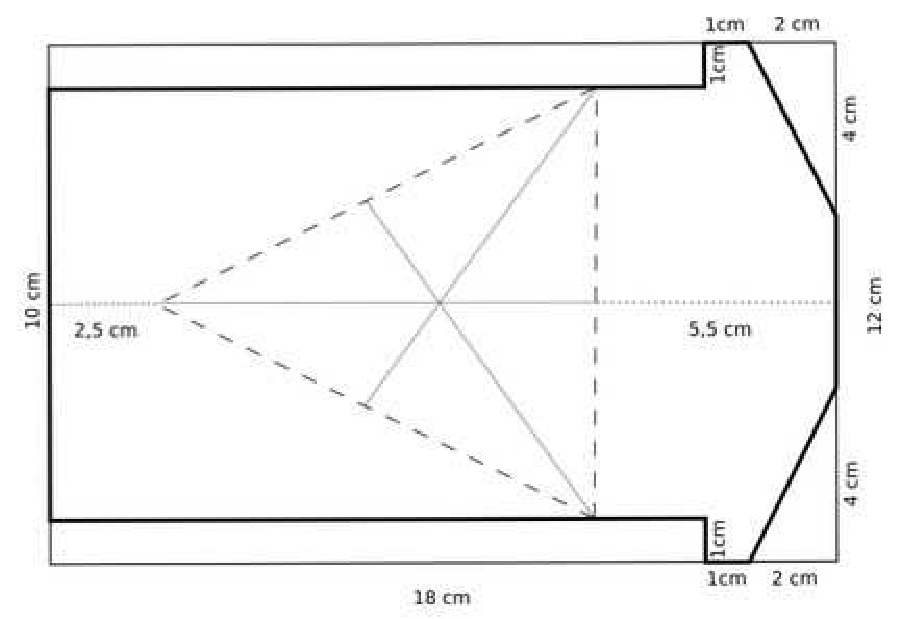
\includegraphics[width=\linewidth]{figure-01.pdf}
    \subcaption{}
    \end{minipage}
    \hfill
    \begin{minipage}{0.47\textwidth}
    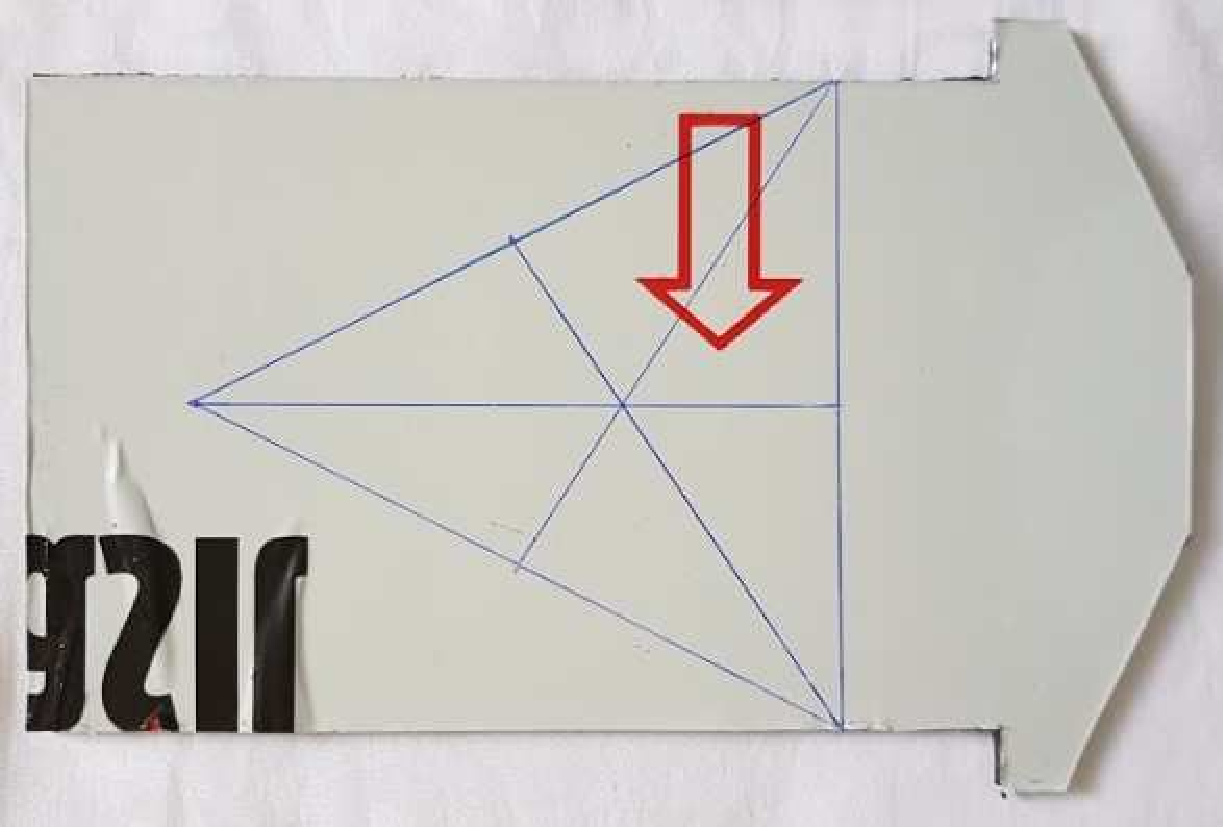
\includegraphics[width=\linewidth]{figure-02.pdf}
    \subcaption{}
    \end{minipage}
    \caption{Chassi.}
    \label{fig01}
    \source{Acervo dos autores.}
    \end{figure}

    \end{enumerate}

    \item Quanto aos motores, retire dois conjuntos de engrenagens, polias e motores presentes em leitoras de DVD de computadores.
    \begin{enumerate}
    \item[2.1] Com uma lâmina para arco de serra, retire os componentes como indicado na \Cref{fig02}.

    \begin{figure}[h!]
    \begin{minipage}{0.47\textwidth}
    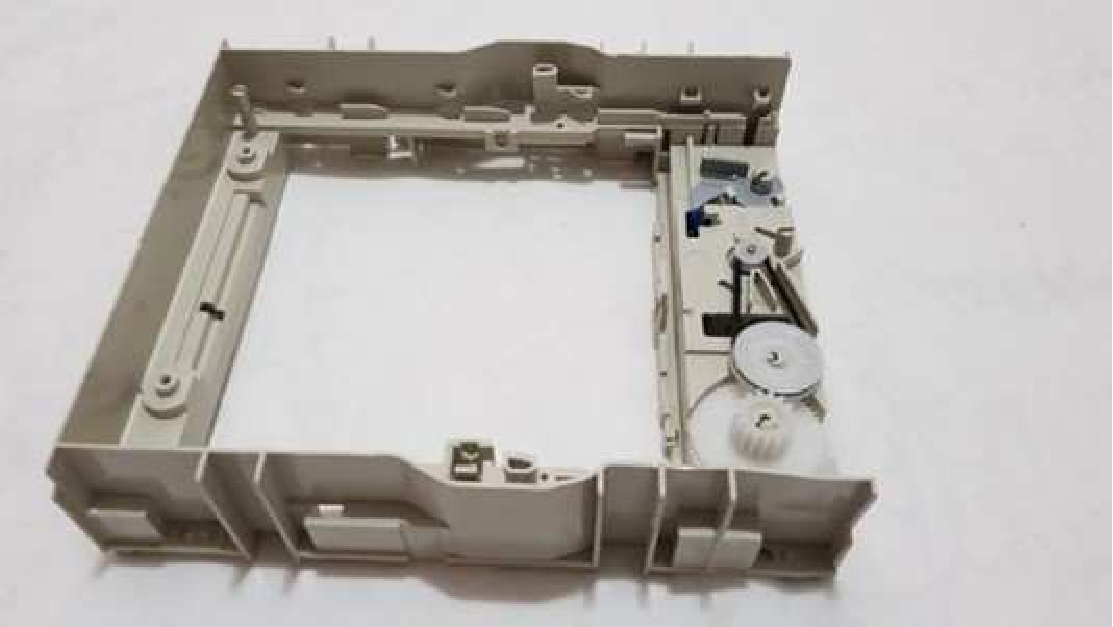
\includegraphics[width=\linewidth]{figure-03.pdf}
    \subcaption{}
    \end{minipage}
    \hfill
    \begin{minipage}{0.47\textwidth} 
    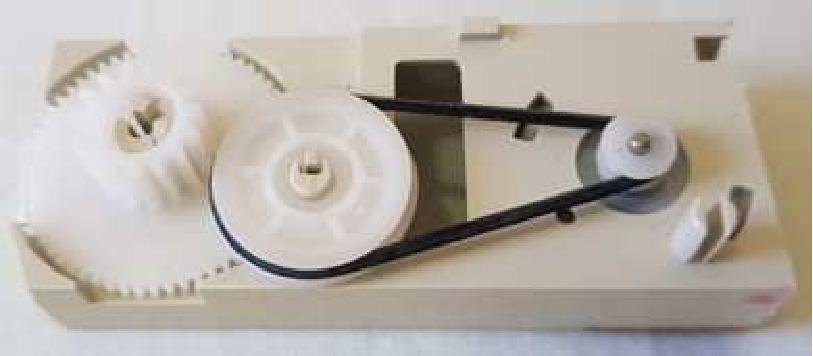
\includegraphics[width=\linewidth]{figure-04.pdf}
    \subcaption{}
    \end{minipage}
    \caption{Engrenagens e motores.}
    \label{fig02}
    \source{Acervo dos autores.}
    \end{figure}
    
    \item[2.2] Desenhe dois círculos de raio 2,5cm em um chinelo. Recorte-os para
    confeccionar as rodas traseiras. Prenda cada círculo em um parafuso com
    rosca, fixe-o na furadeira e, a partir de autorrotação, faça o acabamento
    com uma lixa. Com prego, faça sulcos nas rodas para garantir maior atrito.
    Fixe essas rodas com supercola nas engrenagens, conforme \Cref{fig03}. Caso for
    necessário, as rodas podem ser fixadas com uma estrutura de eixo,
    utilizando rebites e conectores de chuveiros.

    \begin{figure}[H]
    \begin{minipage}{0.31\textwidth}
    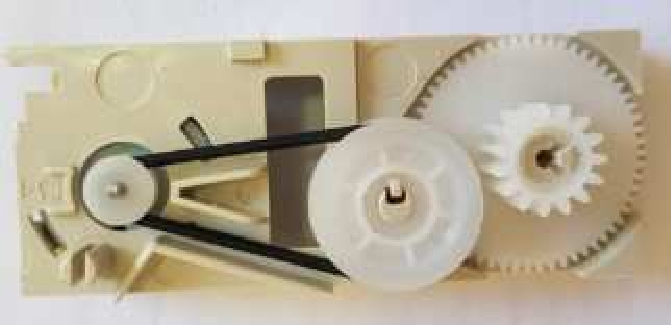
\includegraphics[width=\linewidth]{figure-05.pdf}
    \subcaption{}
    \end{minipage}
    \hfill
    \begin{minipage}{0.31\textwidth} 
    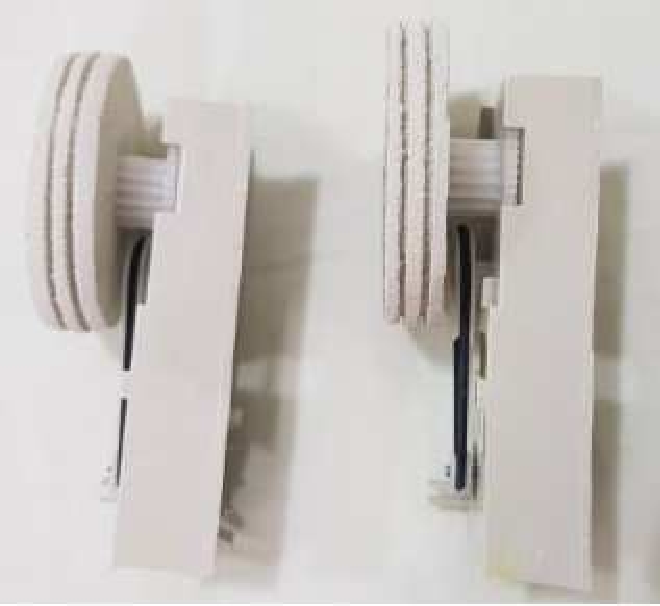
\includegraphics[width=\linewidth]{figure-06.pdf}
    \subcaption{}
    \end{minipage}
    \hfill
    \begin{minipage}{0.31\textwidth} 
    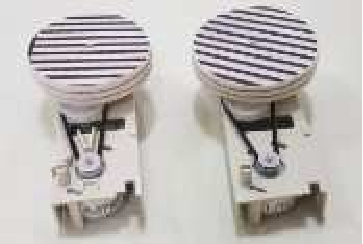
\includegraphics[width=\linewidth]{figure-07.pdf}
    \subcaption{}
    \end{minipage}
    \caption{Fixação das rodas.}
    \label{fig03}
    \source{Acervo dos autores.}
    \end{figure}

    \item[2.3] Fixe as duas estruturas de motor/polias/engrenagens/rodas no chassi
    com supercola ou parafusos e porcas. Cada uma delas deve ser fixada próxima à
    uma das bordas do chassi, de forma que o eixo da roda esteja alinhado ao
    vértice da base do triângulo referência, conforme \Cref{fig04}. 

    \end{enumerate}

    \item Corte o vidro do roll-on labial deixando a esfera presa à base
    cilíndrica, para usá-lo como roda dianteira. A altura total deve ser
    aproximadamente 4cm (a altura da frente do AGV deve ser compatível com a da
    traseira). Fixe a roda no chassi, com o centro alinhado ao vértice superior
    do triângulo referência, conforme \Cref{fig04}.

    \begin{figure}[h!]
    \begin{minipage}{0.47\textwidth}
    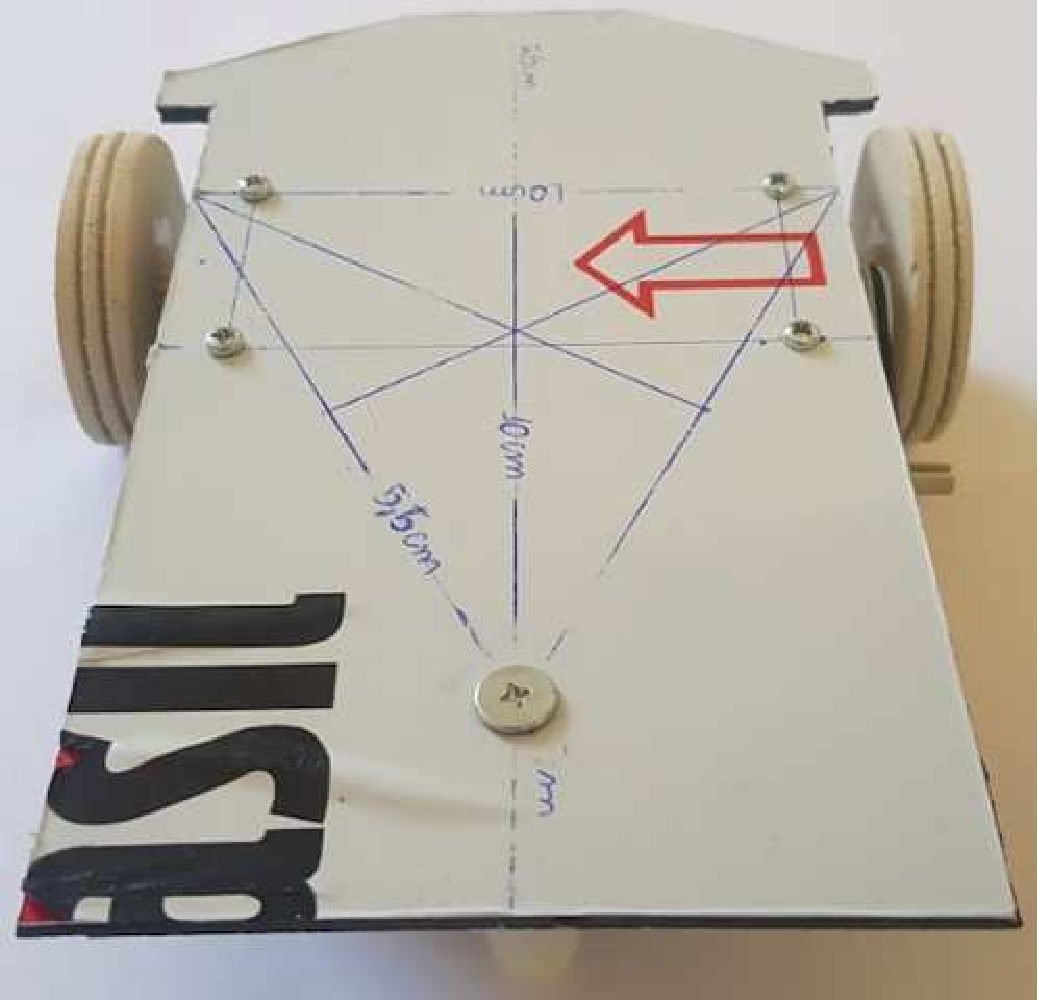
\includegraphics[width=\linewidth]{figure-08.pdf}
    \subcaption{}
    \end{minipage}
    \hfill
    \begin{minipage}{0.47\textwidth} 
    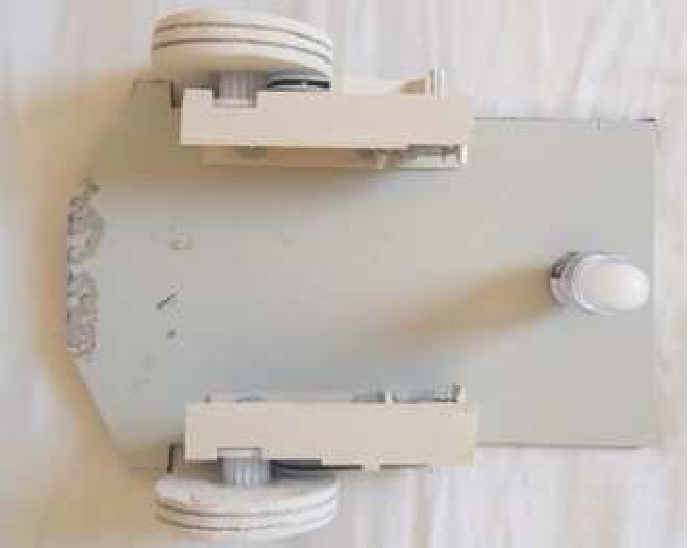
\includegraphics[width=\linewidth]{figure-09.pdf}
    \subcaption{}
    \end{minipage}
    \caption{Estrutura do AGV.}
    \label{fig04}
    \source{Acervo dos autores.}
    \end{figure}
 
\end{enumerate}


Construída a parte estrutural, segue-se para parte eletrônica do robô.


\subsection{Construção da parte eletrônica do AGV}\label{sec-constr-eletr}
O circuito eletrônico\footnote{Todo circuito pode também ser simulado em uma
protoboard ou nos softwares Tinkercad ou Proteus 8.} do AGV, para cada roda,
será separado em três partes, a saber LED-resistor, LDR-potenciômetro e
motor-potenciômetro-transistor. Ressalta-se que a fonte de alimentação e a
chave liga/desliga são compartilhadas pelas três partes. Será feita uma breve
descrição dos circuitos, os quais serão detalhados na sequência.

O circuito LED-resistor tem como objetivo iluminar a trajetória do robô,
propiciando uma leitura adequada do LDR. Enquanto o LED possui a atribuição
iluminar, o resistor evita que o LED se queime, promovendo resistência à
corrente e, por conseguinte, à tensão elétrica.

O circuito LDR-potenciômetro trabalha com o objetivo de manter o veículo na
trajetória. No momento em que um LDR focaliza a linha preta, a tensão do
respectivo circuito diminui, liberando uma quantidade menor corrente e tensão
para o transistor e, consequentemente, para o motor correspondente. Assim,
causa a baixa de velocidade do motor e a correção da trajetória.

O circuito motor-potenciômetro-transistor é o responsável por promover a
locomoção do robô. O transistor regula a quantidade de tensão no motor. O
potenciômetro permite correções nas altas tensões que passariam para o motor,
evitando velocidades muito altas e imprecisão do AGV. A velocidade de rotação do motor depende da tensão nele.


\subsubsection{Primeiro circuito do AGV: LED-resistor}\label{sec-prim-circ}
O LED é um diodo que converte energia elétrica em luz. Só permite que a
corrente flua em uma direção, do lado positivo - ânodo - para o lado negativo -
cátodo (atenção ao design interno das colunas do LED na \Cref{fig05b}). Nesta
pesquisa foram utilizados os LED retratados da \Cref{fig05a}.

\begin{figure}[h!]
\begin{minipage}{0.27\textwidth}
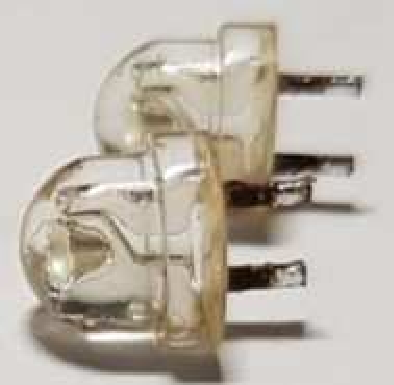
\includegraphics[width=\linewidth]{figure-10.pdf}
\subcaption{}\label{fig05a}
\end{minipage}
\hfill
\begin{minipage}{0.47\textwidth} 
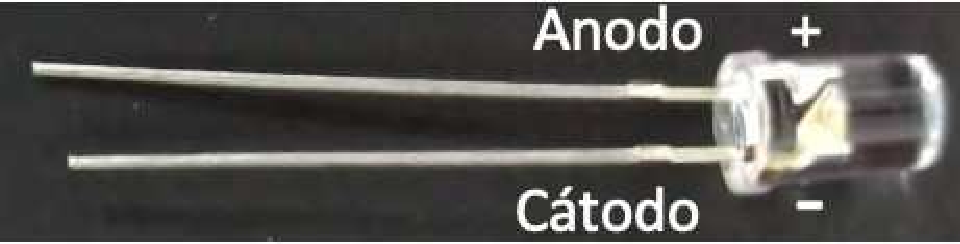
\includegraphics[width=\linewidth]{figure-11.pdf}
\subcaption{}\label{fig05b}
\end{minipage}
\caption{LED.}
\label{fig05}
\source{Acervo dos autores.}
\end{figure}

O resistor, \Cref{fig06}, é um componente que oferece uma oposição à passagem de
corrente elétrica através de seu material. Essa oposição é denominada
resistência elétrica. O resistor não possui polaridade, ou seja, não tem lados
positivo e negativo.

\begin{figure}[htbp]
\centering
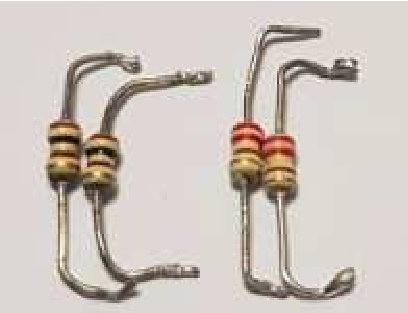
\includegraphics[width=0.25\textwidth]{figure-12.pdf}
\caption{Resistores.}
\label{fig06}
\source{Acervo dos autores.}
\end{figure}

O primeiro circuito é composto por (a) fonte de alimentação com tensão $V_{FA} = 9V$
(bateria de 9V), (b) chave liga/desliga, (c) resistor e (d) LED,
conforme \Cref{fig07}.

\begin{figure}[htbp]
\centering
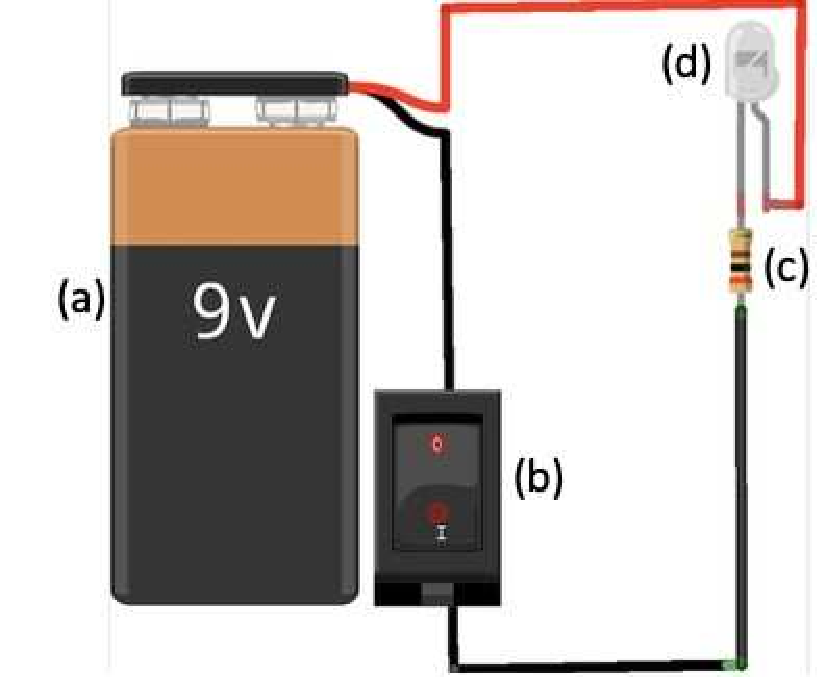
\includegraphics[width=0.25\textwidth]{figure-13.pdf}
\caption{Primeiro Circuito.}
\label{fig07}
\source{Acervo dos autores.}
\end{figure}

Os LED são de 3V e corrente máxima de $20mA = 0,02A$. O valor nominal do
resistor, que será calculado na \Cref{sec-escolha-R}, deve ser $300\Omega$, o qual pode ser
substituído por um resistor de $220\Omega$ e um de $100\Omega$ colocados em série.


\subsubsection{Segundo circuito do AGV: LDR-potenciômetro}\label{sec-seg-circ}
Potenciômetro, \Cref{fig08}, é um componente que possui resistência elétrica
ajustável. Geralmente, é um resistor de três terminais, onde a conexão central
é deslizante e manipulável. Serão utilizados potenciômetros lineares (sufixo B
ao final do código).

\begin{figure}[htbp]
\centering
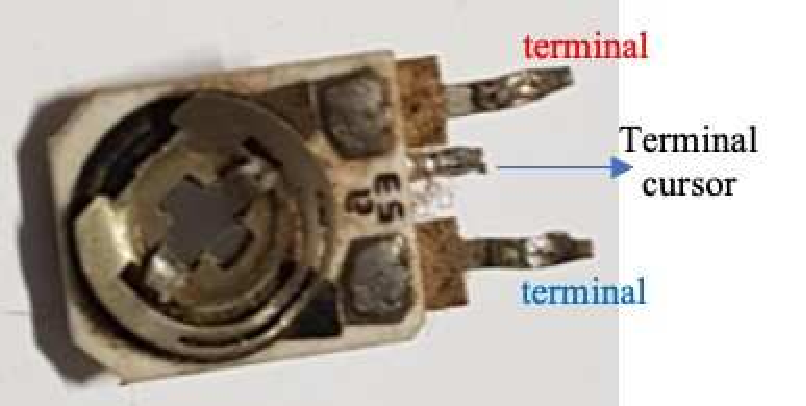
\includegraphics[width=0.25\textwidth]{figure-14.pdf}
\caption{Potenciômetro.}
\label{fig08}
\source{Acervo dos autores.}
\end{figure}

LDR, \Cref{fig09}, é um resistor cuja resistência varia conforme a intensidade da
luz que incide sobre ele, o qual não possui polaridade nos terminais. Quanto
maior a intensidade da luz mais a resistência diminui. Optou-se por utilizar um
LDR de 5mm.

\begin{figure}[htbp]
\centering
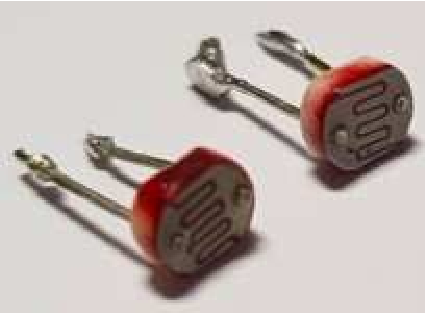
\includegraphics[width=0.25\textwidth]{figure-15.pdf}
\caption{LDR.}
\label{fig09}
\source{Acervo dos autores.}
\end{figure}

O segundo circuito é composto pela (a) fonte de alimentação, (b) chave
liga/desliga, (e) potenciômetro e (f) LDR, conforme \Cref{fig10}.

\begin{figure}[htbp]
\centering
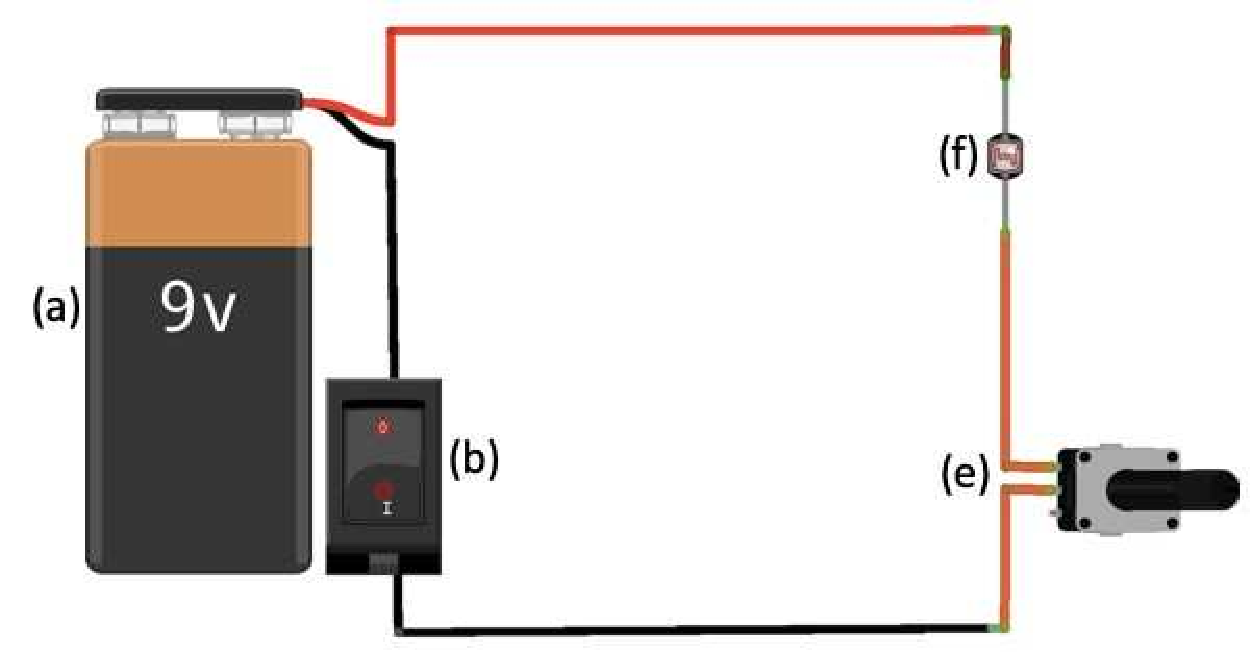
\includegraphics[width=0.5\textwidth]{figure-16.pdf}
\caption{Segundo Circuito.}
\label{fig10}
\source{Acervo dos autores.}
\end{figure}

Os potenciômetros desse circuito devem ser ajustados de acordo com os
transistores (\Cref{sec-terceiro-circ}) utilizados no AGV, conforme as seguintes faixas

\begin{table}[htpb]
\caption{Legenda da tabela do documento modelo da revista \emph{Texto Livre}.}
\label{tbl-tabela-01}
\begin{tabular}{
     >{\raggedright\arraybackslash}p{0.2\textwidth}
     >{\raggedright\arraybackslash}p{0.2\textwidth}
     >{\raggedright\arraybackslash}p{0.4\textwidth}
}
\toprule 
\multicolumn{2}{l}{Transistor} & Potenciômetro ou resistor \\
NPN & PNP & \begin{tabular}[c]{@{}l@{}}Faixa de variação para funcionamento do\\ circuito\end{tabular} \\
\midrule
\begin{tabular}[c]{@{}l@{}}TIP’s 102, 120 e\\ 122\end{tabular} &  & \multirow{2}{*}{$200\Omega$ à $600\Omega$} \\
 & \begin{tabular}[c]{@{}l@{}}TIP’s 105 e\\ 107\end{tabular} &  \\
 \midrule
  & \begin{tabular}[c]{@{}l@{}}BD: 140 e\\ 136\end{tabular} & \multirow{2}{*}{$120\Omega$ à $330\Omega$} \\
  BD 135 e 139 &  & \\
\bottomrule
\end{tabular}
\source{Fonte da tabela.}
\end{table}



\FloatBarrier 

\subsubsection{Terceiro circuito do AGV: motor-potenciômetro-transistor}\label{sec-terceiro-circ}
O terceiro circuito é o programador do AGV. Existem vários tipos de
transistores, o que propicia o desafio de descobrir as alterações necessárias
no circuito para cada modelo. Serão tratados neste artigo somente transistores
NPN e PNP, nos modelos BD e TIP.

O transistor, \Cref{fig11}, é um dispositivo semicondutor usado para amplificar ou
oscilar sinais eletrônicos e potência elétrica. Também pode ser usado como
chave eletrônica. É composto por três terminais, base, coletor e emissor. A
informação de qual terminal é base, coletor ou emissor deve ser verificada no
datasheet do componente.

\begin{figure}[htbp]
\centering
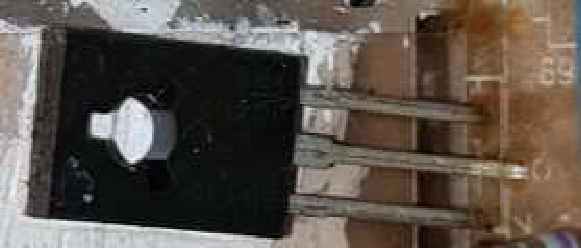
\includegraphics[width=0.25\textwidth]{figure-17.pdf}
\caption{Transistor.}
\label{fig11}
\source{Acervo dos autores.}
\end{figure}

É possível comparar o funcionamento do transistor a uma torneira de água, na
qual a regulação da quantidade de água que sai, depende do quanto se abre a
válvula. No caso do transistor, será regulada, pela base, a quantidade de
corrente elétrica. Na \Cref{fig12}, pode-se visualizar em esquema as diferenças
dos transistores NPN e PNP.

\begin{figure}[h!]
\centering
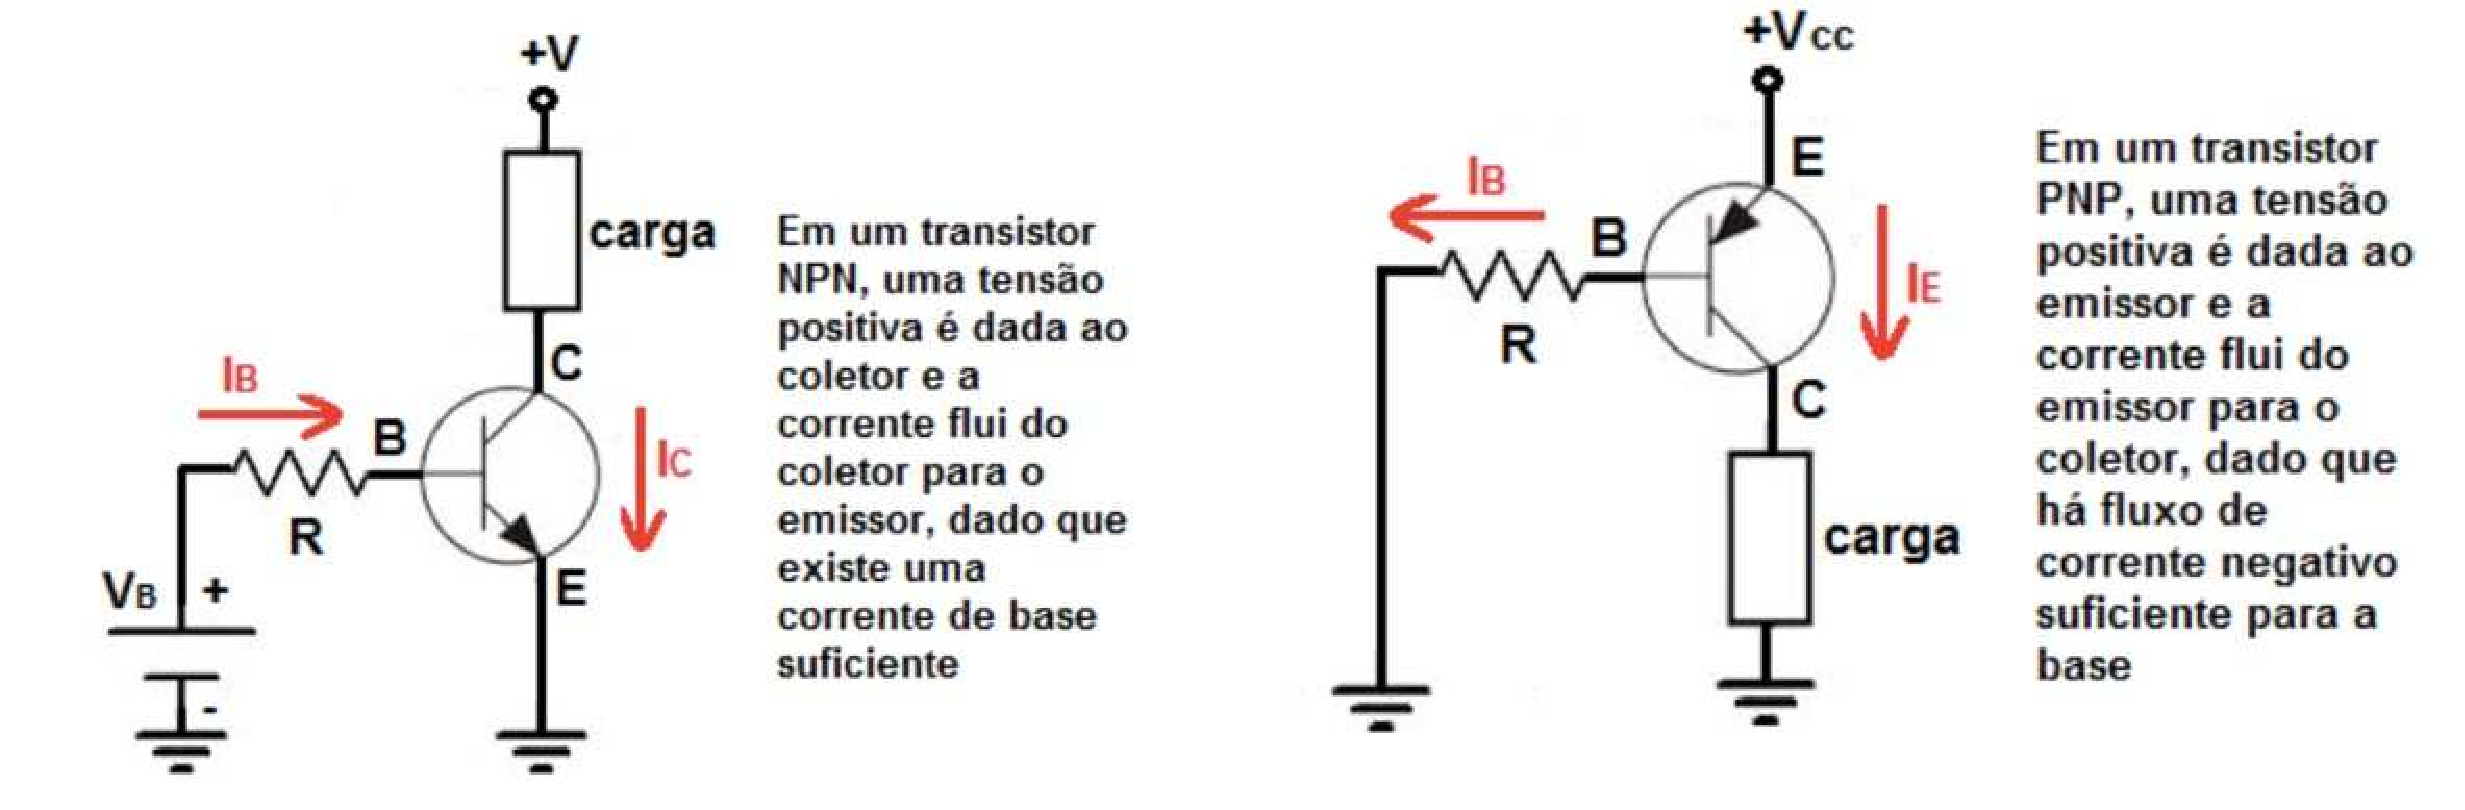
\includegraphics[width=0.75\textwidth]{figure-18.pdf}
\caption{Esquema de transistores NPN e PNP.}
\label{fig12}
\source{Aprender sobre eletrônicos \url{http://www.learningaboutelectronics.com/Artigos/Diferenca-entre-transistores-NPN-e-PNP.php}.}
\end{figure}
 
Um motor DC (direct current) é um motor elétrico rotativo que converte energia
elétrica de corrente contínua em energia mecânica. A velocidade de um motor DC
pode ser controlada em uma ampla faixa, usando uma tensão de alimentação
variável ou alterando a força da corrente em seus enrolamentos de campo. Esses
motores revertem a rotação quando se troca a polarização. Foi utilizado um
motor que sai do repouso com uma tensão maior que 2,8V, conforme informação do
datasheet\footnote{Disponível em:
\url{https://datasheetspdf.com/parts/RF-300EA-1D390.pdf?id=917203}.}.

O conjunto de motores/polias/engrenagens não precisam ser idênticos, porém é
necessário que os motores tenham tensões próximas e as engrenagens devem ter o
mesmo número de dentes.

O terceiro circuito é composto por (a) fonte de alimentação, (b) chave
liga/desliga, (g) motor DC (h) potenciômetro e (i) transistor. Na \Cref{fig13}
estão esquematizados os três circuitos integrados, com (a) fonte de
alimentação, (b) chave liga/desliga, (c) resistor, (d) LED, (e) potenciômetro,
(f) LDR, (g) motor DC, (h) potenciômetro e (i) transistor. Para este esquema
foi considerado um transistor NPN BD. Para trabalhar com um transistor PNP
deve-se inverter a polarização do circuito, o que pode inferir da \Cref{fig13}
(cuidado com a polarização do LED em caso de inversão).

\begin{figure}[h!]
\centering
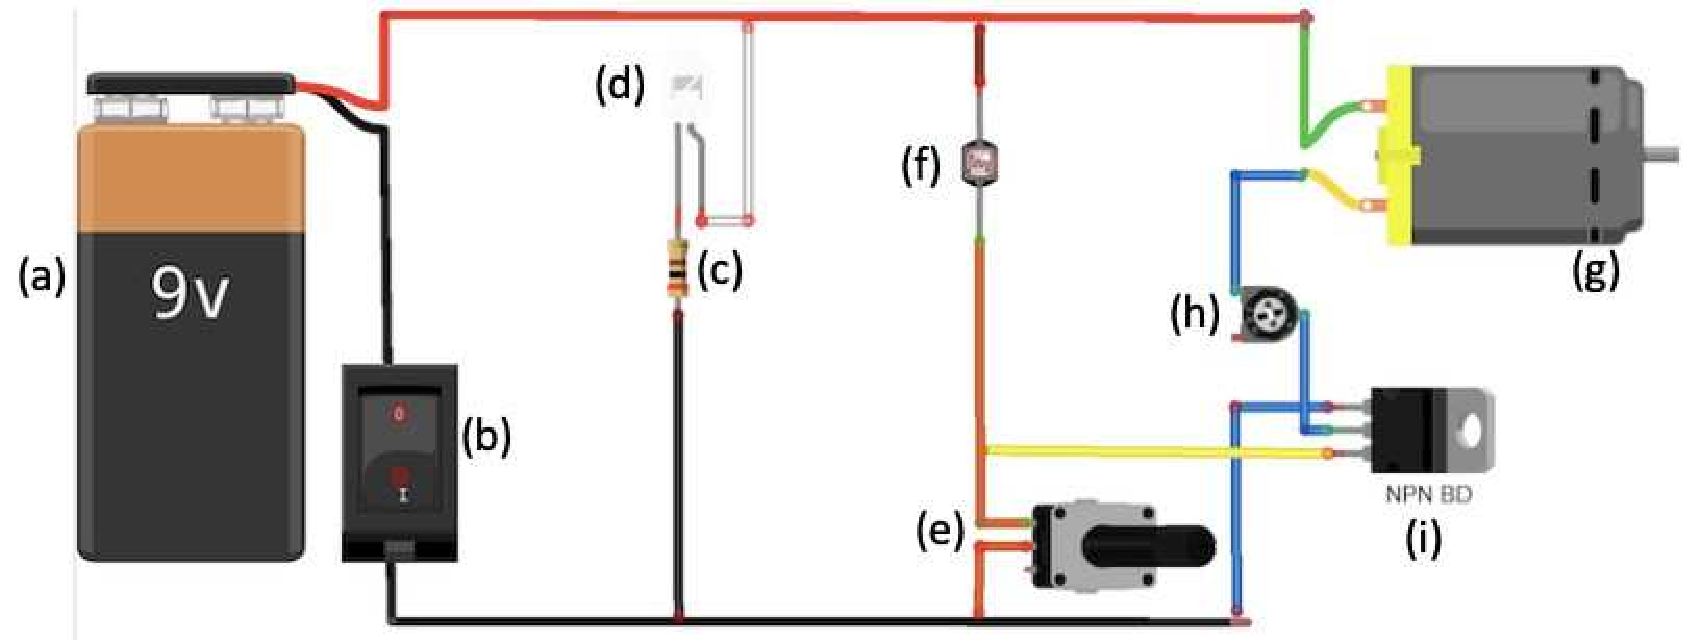
\includegraphics[width=0.5\textwidth]{figure-19.pdf}
\caption{Terceiro Circuito.}
\label{fig13}
\source{Acervo dos autores.}
\end{figure}

Entre segundo e o terceiro circuitos há uma leitura de corrente, essa leitura
realizada pela base do transistor que irá controlar o AGV. Assim, um fio entre
o LDR e potenciômetro é ligado à base do transistor, regulando-o
eletronicamente.

Para fixação dos componentes eletrônicos no robô, inicia-se pelo LDR que deve
ser colocado a uma altura de 1cm do chão, dentro de um canudinho coberto com
fita isolante preta. A iluminação, feita por um LED de alto brilho, também deve
ser colocada a uma altura de 1cm do chão e 1cm de distância do LDR. Esses
componentes podem ser acoplados ao chassi com supercola na parte inferior do
robô, conforme indicado na \Cref{fig14}. Esta configuração foi utilizada para que
o AGV possa seguir uma trajetória formada por fita isolante dupla de cor preta
(3,5cm de largura) em uma base clara.

\begin{figure}[h!]
\centering
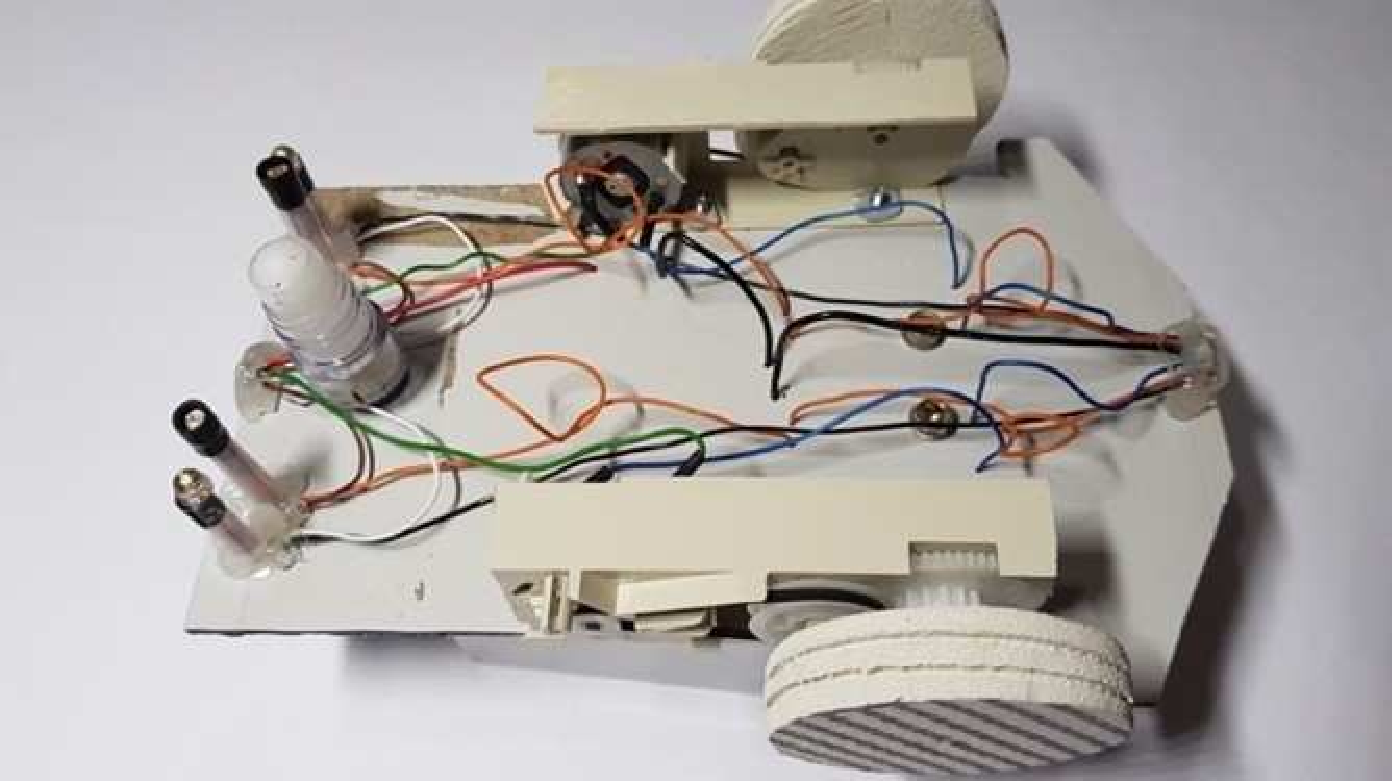
\includegraphics[width=0.5\textwidth]{figure-20.pdf}
\caption{Parte inferior do AGV.}
\label{fig14}
\source{Acervo dos autores.}
\end{figure}

Na parte superior, estabiliza-se a bateria no chassi, colocando-a em uma
posição que propicie estabilidade ao robô. O ideal é usar como referência o
centro de massa do triângulo, conforme \Cref{fig01}. Fixe a chave liga/desliga, os
transistores e potenciômetros em uma placa de plástico rígido e depois cole a
placa no chassi, conforme \Cref{fig15}.

\begin{figure}[H]
\centering
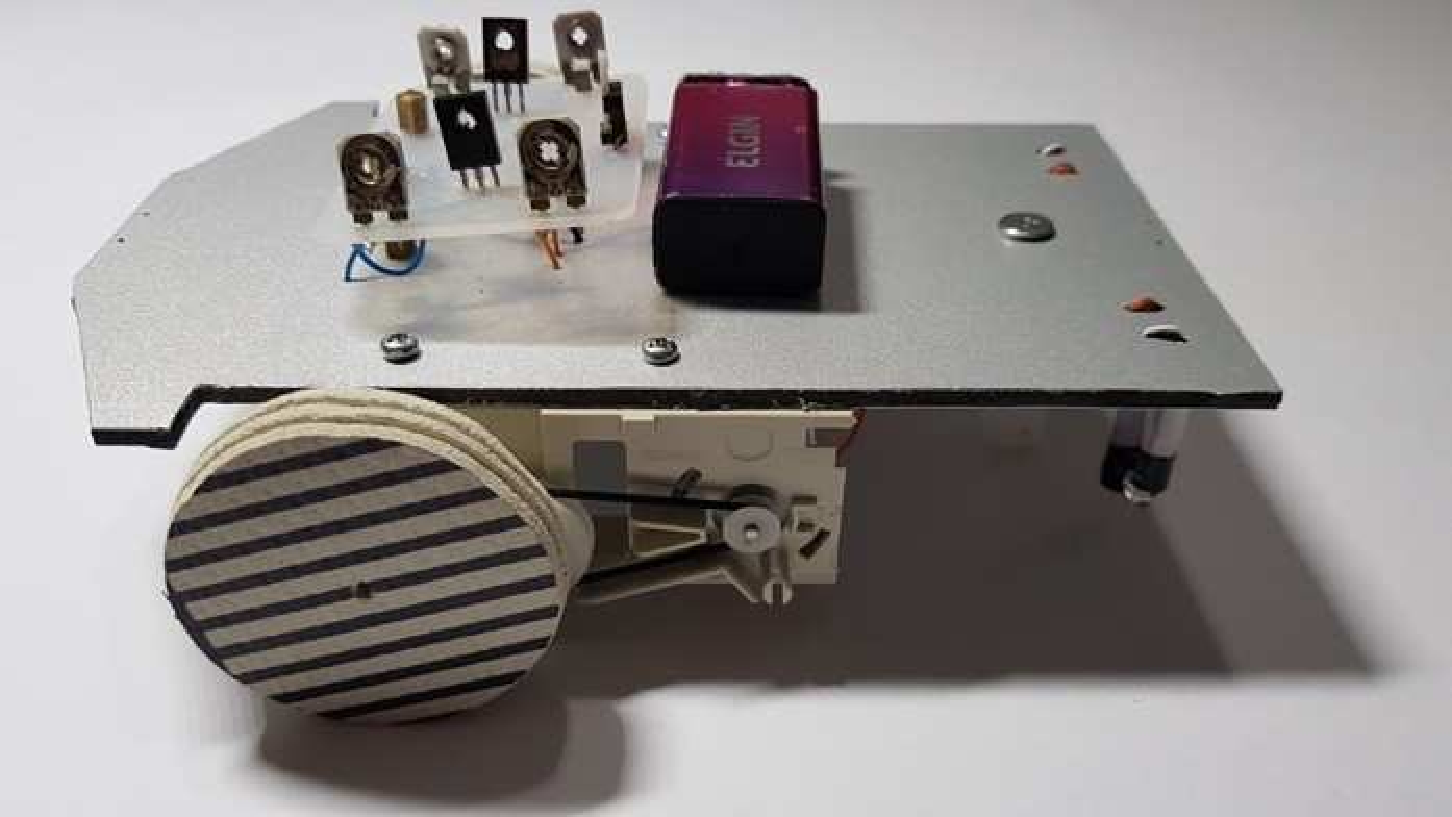
\includegraphics[width=0.5\textwidth]{figure-21.pdf}
\caption{Parte superior do AGV.}
\label{fig15}
\source{Acervo dos autores.}
\end{figure}

Segue na \Cref{fig16} um esquema para orientar a montagem do circuito no AGV, com
indicação dos furos para passagem dos fios. Todos os fios devem ser soldados
aos componentes eletrônicos.

\begin{figure}[H]
\begin{minipage}{0.47\textwidth}
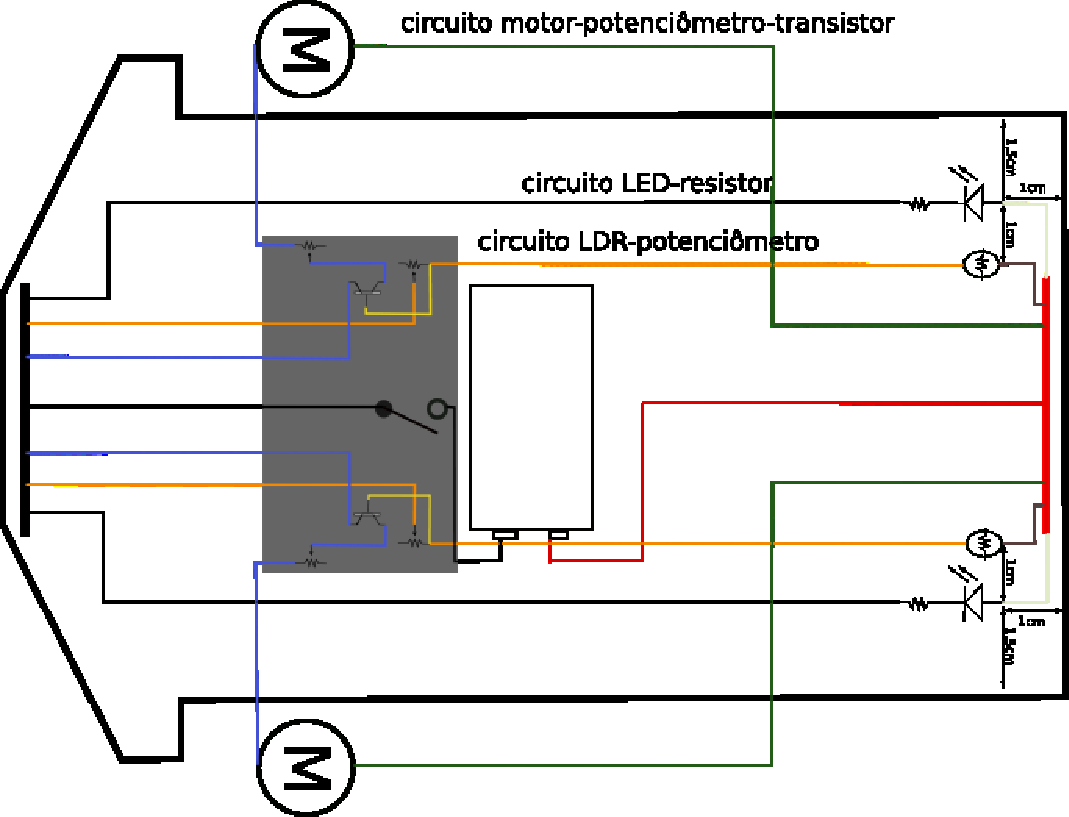
\includegraphics[width=\linewidth]{figure-22.pdf}
\subcaption{}
\end{minipage}
\hfill
\begin{minipage}{0.47\textwidth} 
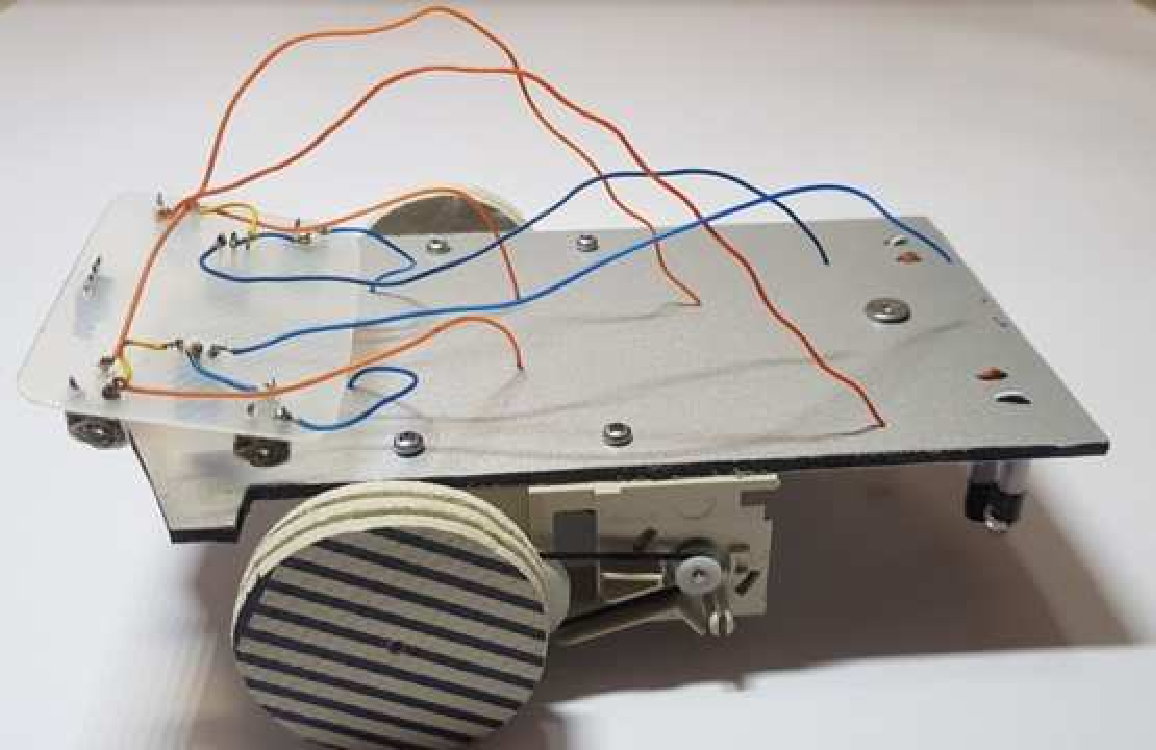
\includegraphics[width=\linewidth]{figure-23.pdf}
\subcaption{}
\end{minipage}
\caption{Circuitos no AGV.}
\label{fig16}
\source{Acervo dos autores.}
\end{figure}

A construção do AGV está concluída e o processo de desenvolvimento da pesquisa
será relatado a seguir.


\subsection{O Desenvolvimento da Pesquisa}\label{sec-desenvolvimento}
Inicialmente, foi construído um robô seguidor de linha utilizando as peças
relacionadas em \textcite{thenorio}. O valor gasto para a aquisição delas foi R\$
113,40. Posteriormente, iniciou-se a busca por respostas para o seguinte
questionamento “Quais adaptações podem ser feitas na proposta de construção de
um seguidor de linha, para se trabalhar na perspectiva livre, mantendo a
eficiência e a eficácia, e estabelecer uma SD envolvendo conteúdos de
Matemática e Física neste processo?”. Esta investigação foi conduzida baseada
na experimentação de componentes de sucatas que pudessem substituir as peças
compradas, bem como na exploração da Matemática e Física subjacente. Neste
processo, foram encontrados os componentes citados na quarta coluna da \Cref{tab01}.
Alguns problemas ocorreram neste processo e foram feitas adaptações para
obter melhores resultados na performance do robô.

Nos experimentos executados, para o chassi foram utilizados 3 materiais
distintos, pasta de plástico, capa rígida de caderno e ACM. O plástico, por ser
muito flexível, não produziu o efeito desejado, os outros dois materiais foram
boas opções. Além disso, nesta etapa foram pensados os conteúdos que
possivelmente seriam abordados, de onde surgiu a necessidade de montar a \Cref{fig01}
para execução da SD.

Quanto aos motores, foram testados motores DC (de impressora) que eram velozes,
porém não possuíam força suficiente para movimentar o robô. Portanto, foi
necessária a utilização de conjuntos de engrenagens/polias/motores presentes em
leitoras de DVD de computadores, o que propiciou um movimento mais preciso do
robô. Esta alteração possibilitou a exploração de diversos conteúdos de
Matemática e Física na SD.

A montagem da parte eletrônica foi feita, inicialmente, sem separações. A
partir das experimentações, concluiu-se que a divisão em 3 partes facilitaria o
entendimento, bem como a elaboração da SD. Foi elaborado um esquema, \Cref{fig16},
para montagem das partes do circuito. No segundo circuito foram testados tanto
potenciômetros quanto resistores para estabelecer uma resistência elétrica.
Apesar de serem opções funcionais, a descrição do circuito foi feita com base
no potenciômetro. O terceiro circuito era composto por motor-transistor. Foram
testados e validados diversos tipos de transistores NPN e PNP, os quais estão
elencados na \Cref{tbl-tabela-01}, a fim de facilitar a procura do componente em sucatas.
Foram utilizados motores de 5.9V, por serem mais fáceis de serem encontrados em
sucatas. Após os testes, optou-se pela inserção de potenciômetros entre os
transistores e motores para proporcionar maior precisão ao movimento do robô.
Contudo, se os motores forem substituídos por outros com tensão menor ou igual
a 3V (menos comuns), é possível reduzir a tensão da fonte de alimentação para
quatro pilhas, 4.8V, e o potenciômetro torna-se dispensável. A montagem da
parte eletrônica do robô também foi trabalhada na SD.

Sobre a escolha do resistor no circuito LED-resistor, na primeira versão, foi
utilizado um resistor de $220\Omega$. Devido às variações de corrente e tensão que
acontecem na prática, o robô funcionou sem problemas. Contudo, ao trabalhar com
modelos matemáticos, os quais não englobam todas as variáveis, foi detectado
que, em condições ideais, esta resistência não seria suficiente, podendo
danificar o LED ou encurtar sua vida útil. Por meio da simulação no software
\emph{Tinkercad} este fato foi corroborado. Consequentemente, o robô foi ajustado para
possibilitar a construção de atividades na SD.

Portanto, foi montado um seguidor de linha, com peças compradas, com base em
experiências de outros autores. Posteriormente, foram feitos dois experimentos
com componentes de sucata, com foco em estabelecer atividades que explorassem a
Matemática e Física, para composição de uma SD. Na próxima seção, estão
descritas as atividades elaboradas a partir da vivência das experiências aqui
relatadas.

\section{Aprendizagens possíveis durante a construção da estrutura do AGV}\label{sec-aprendizagens}
A Robótica Educacional é uma ferramenta que possibilita resolver problemas
matemáticos e interdisciplinares com a utilização de hardware e software,
evidenciando a aplicabilidade da Matemática e da Física. Vale ressaltar que
nesta abordagem, assume-se a perspectiva de que educar é muito mais do que
treinar pessoas para o uso das novas tecnologias, “trata-se de formar os
indivíduos para aprender a aprender de modo a serem capazes de lidar
positivamente com a contínua e acelerada transformação da base tecnológica”
\cite[p. 45]{brasil2000}.

Esse viés de pensamento é essencial na obtenção de resultados em contrapartida
dos problemas sociais gerados pelos avanços tecnológicos. Existem pesquisas que
relatam os impactos da tecnologia na sociedade, por exemplo no O Globo, “UnB
mostra que 30 milhões de empregos serão substituídos por robôs até 2026”
\cite{carvalho2019}. Uma maneira de amenizar esses problemas é formar pessoas
capazes de se adaptar rapidamente às exigências do mercado, com conhecimentos
sobre software e hardware, além de adequar as metodologias para o ensino e
aprendizagem de Matemática que é base essencial para a tecnologia.

A construção deste robô é uma oportunidade de abordar diversos conceitos
matemáticos e físicos de forma significativa para os envolvidos, bem como
instigá-los para a aprendizagem de conceitos de eletrônica e computação. Nesta
seção será evidenciada a Matemática e a Física subjacentes.

O projeto é muito importante para que se construa um AGV eficiente e eficaz,
pois esse modelo não tem um volante. Neste caso, as rodas com tração são fixas
e o giro do corpo do robô pode ser induzido de duas formas, ou pela interrupção
de um dos motores enquanto o outro permanece em movimento, ou por velocidades
diferentes em cada uma das rodas. A terceira roda, ou eixo fixo, facilita as
manobras. Ademais, a fim de promover a estabilidade sobre as 3 rodas é
necessário que o peso esteja bem distribuído.


\subsection{Conceitos geométricos e unidades de medida}\label{sec-conceitos}
Inicialmente, é possível trabalhar figuras planas para a escolha do modelo do
chassi. Outro conceito importante é o de centro de massa, o qual pode ser
trabalhado no triângulo referência. É o centro de massa deste triângulo que
será usado para colocar a bateria, o componente de maior massa do robô.
Portanto, é possível trabalhar conceitos como unidades de medida de massa,
triângulos, triângulos isósceles, vértices, lados, lado oposto a um vértice,
unidades de medida de comprimento, ponto médio de um segmento, mediana,
intersecção de semirretas e baricentro (centro de massa), dentre outros.
Posteriormente, ao construir as rodas, é possível trabalhar os conceitos de
círculo, circunferência, diâmetro, raio e comprimento de circunferência. No
desenvolvimento dessas atividades pode-se abordar as possíveis relações, por
exemplo sobre o comprimento dos segmentos de reta estabelecidos na mediana a
partir da determinação do baricentro.

A partir do centro de massa inicia-se a distribuição dos componentes. Neste
momento podem ser abordados os conceitos de design e aerodinâmica, reforçando a
necessidade de utilização de conhecimentos científicos, em particular
matemáticos, para tomar decisões na construção de tecnologias, minimizando os
testes. Os testes são importantes, pois são hipóteses a serem provadas e nesse
processo há aprendizagem, contudo é preciso valorizar a pesquisa na solução de
um problema.


\subsection{Proporcionalidade, função linear e outros conceitos}\label{sec-proporcionalidade}
Outra fase que propicia a abordagem de conteúdos matemáticos é trabalhar com
motores/polias/engrenagens. Pode-se explorar proporcionalidade, função linear e
outros conceitos, desmontando um conjunto como o indicado na \Cref{fig02}.

É importante abordar que os motores utilizados possuem alta velocidade e pouca
força. Esta característica não é muito interessante, pois a força pode não ser
suficiente para movimentar o robô e com grande velocidade perde-se precisão no
movimento, principalmente por não haver volante. Então, surge a primeira
dificuldade, ganhar torque e reduzir as altas velocidades dos motores. O ideal
é que a rotação das rodas fique abaixo de 250 RPM. A solução é utilizar um
conjunto de polias/engrenagens, sendo uma polia pequena fixada no motor ($P_1$),
uma polia grande ($P_2$) acoplada a uma engrenagem pequena ($E_2$) e uma engrenagem
maior ($E_1$) acoplada à roda, conforme \Cref{fig17}. Segue uma proposta de abordagem
dos conteúdos.

\subsubsection{Primeira atividade}\label{sec-primeira-atividade}
Nessa atividade é possível trabalhar conceitos como comprimento da
circunferência, raio, grandezas diretamente proporcionais, frações, números
decimais, funções lineares, domínio e imagem de uma função linear, inversa de
uma função linear, além das operações básicas. O objetivo é encontrar uma
função linear para determinar o número de voltas da $P_2$ em relação ao número
de voltas da $P_1$ e vice-versa.

\begin{enumerate}
\item Recorde/Introduza a definição e a fórmula para calcular o comprimento da circunferência ($C = 2\pi R$).
\item Utilize para demonstração as polias e engrenagens ilustradas na \Cref{fig17}.

    \begin{figure}[h!]
    \begin{minipage}{0.2\textwidth}
    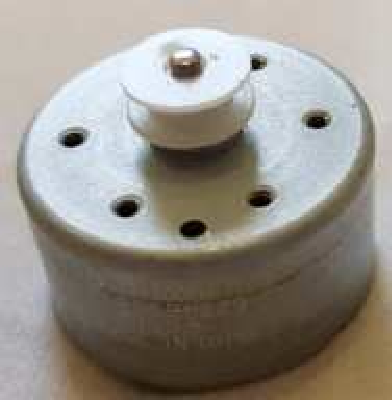
\includegraphics[width=\linewidth]{figure-24.pdf}
    \subcaption{Motor/$P_1$.}\label{fig17a}
    \end{minipage}
    \hfill
    \begin{minipage}{0.2\textwidth} 
    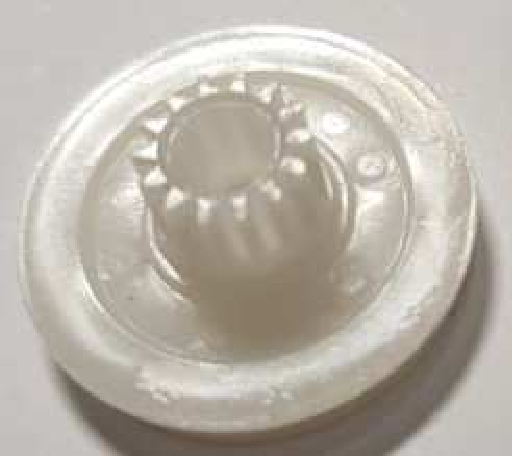
\includegraphics[width=\linewidth]{figure-25.pdf}
    \subcaption{$P_2/E_2$.}\label{fig17b}
    \end{minipage}
    \hfill
    \begin{minipage}{0.2\textwidth} 
    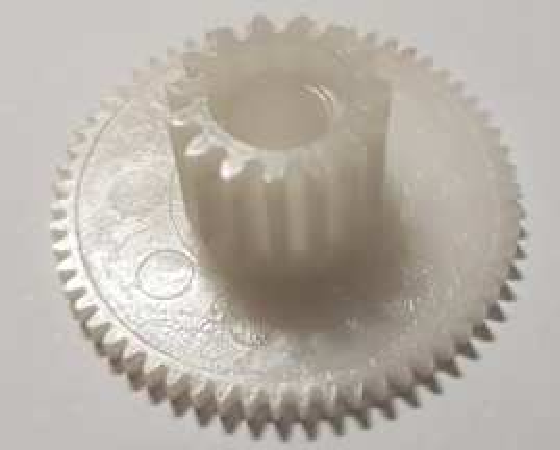
\includegraphics[width=\linewidth]{figure-26.pdf}
    \subcaption{$E_1$ e engrenagem onde será conectada a roda.}\label{fig17c}
    \end{minipage}
    \hfill
    \begin{minipage}{0.33\textwidth} 
    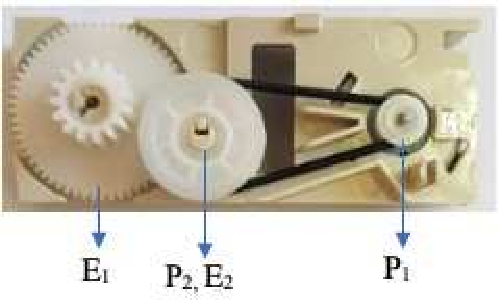
\includegraphics[width=\linewidth]{figure-27.pdf}
    \subcaption{$P_1$ e $P_2$ conectadas por correia $E_1$ e $E_2$ em contato.}\label{fig17d}
    \end{minipage}
    \caption{Polias e engrenagens.}
    \label{fig17}
    \source{Acervo dos autores.}
    \end{figure}

    \begin{enumerate}
    \item[2.1] Calcule o raio de $P_1$ (0,27cm) e seu comprimento ($\approx$ 1,69cm).
    \item[2.2] Calcule o raio de $P_2$ (0,9cm) e seu comprimento ($\approx$ 5,65cm).
    \item[2.3] Relembre/introduza o que são grandezas diretamente proporcionais
    utilizando como exemplo o raio e o comprimento da circunferência.
    \item[2.4] Induza os estudantes a perceberem que uma volta completa da $P_2$
    (maior) implica 3,343 rotações da $P_1$, ou equivalentemente, cada rotação
    da $P_1$ implica que $P_2$ gira a fração 1,69/5,65 ($\approx$ 0,299).
    \end{enumerate}

    \item Recorde/introduza a definição de função linear, domínio e imagem.
    Defina uma função para determinar o número de voltas da $P_2$ em relação ao
    número de voltas da $P_1$ e outra para determinar o número de voltas da
    $P_1$ em relação ao número de voltas da $P_2$.

    \begin{align*}
    f_1: \mathbb{R}^{+} \rightarrow \mathbb{R}^{+} && f_{1}^{-1}: \mathbb{R}^{+} \rightarrow \mathbb{R}^{+} \\
    x \rightarrow 0,299x && x \rightarrow 3,343x \nonumber
    \end{align*}

\end{enumerate}



\subsubsection{Segunda atividade}\label{sec-segunda}
Nessa atividade é possível trabalhar funções lineares, domínio e imagem de
funções lineares, inversa de uma função linear, frações, números decimais e
operações básicas. O objetivo é encontrar uma função linear para determinar o
número de voltas da $E_1$ com relação ao número de voltas da $P_2$ e vice-versa.

\begin{enumerate}
\item Chame a atenção para o fato de que a $P_2$ está acoplada a uma engrenagem de
14 dentes (\Cref{fig17b}) e estão centradas no mesmo eixo. Como consequência, a
cada giro da $P_2$ corresponde um giro da $E_2$
\item Enfatize que o giro de $E_2$ movimenta uma engrenagem de 60 dentes
($E_1$ - \Cref{fig17c}), pois as duas estão em contato, conforme \Cref{fig17d}. Nessa
Figura não é possível ver a $E_2$, acoplada à $P_2$. É importante relembrar que a $E_1$
será presa à roda.
\item Induza os estudantes a concluírem que para $E_1$ dar um giro completo a $P_2$
precisa girar 60/14 ($\approx$ 4,285) voltas, ou a cada volta da $P_2$ a $E_1$ gira a fração
14/60 ($\approx$ 0,233).
\item Recorde/introduza a definição de função linear, domínio, imagem.
Introduza uma função para determinar o número de voltas da $E_1$ com relação ao
número de voltas da $P_2$ e outra para determinar o número de voltas da $P_2$
com relação ao número de voltas da $E_1$.

    \begin{align*}
    f_2: \mathbb{R}^{+} &\rightarrow \mathbb{R}^{+} & f_{2}^{-1}: \mathbb{R}^{+} &\rightarrow \mathbb{R}^{+} \\
    x &\rightarrow 0,233x & x &\rightarrow 4,285x \nonumber
    \end{align*}

\end{enumerate}



\subsubsection{Terceira atividade}\label{sec-terceira}

Nesta atividade é possível trabalhar composição de funções lineares, domínio e
imagem de uma função composta, comprimento de uma circunferência, conversão de
unidades de velocidade e operações básicas. O objetivo é calcular a velocidade
que o AGV vai atingir.

\begin{enumerate}
\item\label{itm1sec423} Faça um apanhado sobre composição de funções e introduza a função $f_2 \circ f_1$
    \begin{align*}
    f_2 \circ f_1: \mathbb{R}^{+} &\rightarrow \mathbb{R}^{+}  \\
    x &\rightarrow 0,0696x \nonumber
    \end{align*}

\item Induza os estudantes a concluírem que, a partir da composição das funções
$f_1$ e $f_2$, é possível relacionar a quantidade de giros da roda (giros da
$E_1$) com o número de voltas do motor (giros da $P_1$) e determinar o número
de rotações por minuto (RPM) da roda com respeito ao número de RPM do motor.

\item Solicite que os estudantes calculem o número de RPM da roda, indicando
que o motor gira 3520 RPM com atrito (veja datasheet\footnote{Disponível em:
\url{https://datasheetspdf.com/parts/RF-300EA-1D390.pdf?id=917203}.}). O
professor precisa ficar atento a numeração dos motores e das respectivas
informações nos datasheet. Verifique se todos concluíram que o número de
rotações da roda é, aproximadamente, 245 RPM.

\item Relembre/introduza como calcular o comprimento de uma circunferência e
solicite que calculem o comprimento das rodas ($\approx$ 15,7cm), tendo em
vista que o raio delas é 2,5cm.

\item Induza à conclusão de que o AGV percorrerá 3846cm/min, ou 64,1cm/s.
\end{enumerate}

Infelizmente, na prática há vários outros fatores, como peso do robô, frenagens
dos motores para a correção da trajetória, oscilação da tensão nos motores,
capacidade elétrica da fonte de alimentação, entre outros, que interferem na
quantidade de RPM da roda, como será visto no \Cref{itm6} da \Cref{sec-quarta}.

\subsubsection{Quarta atividade}\label{sec-quarta}
Nesta atividade é possível trabalhar cálculo de velocidade, conversão de
unidades de medida e unidades de velocidade, comprimento da circunferência,
função inversa, números decimais e operações básicas. O objetivo é calcular o
número médio de RPM do motor a partir da distância percorrida pelo AGV. Vale
ressaltar que os valores obtidos, pelos pesquisadores, empiricamente com o robô
é uma média feita a partir das testagens. Além disso, estão citados no trabalho
(entre parênteses) apenas para referência, pois outros robôs, provavelmente,
terão desempenhos diferentes, assim como aconteceu com os dois exemplares
citados no artigo.

\begin{enumerate}
\item Faça os estudantes construírem uma pista, usando fita isolante preta
(dupla 3,5cm de largura) sobre um piso claro ou duas cartolinas chambril,
conforme \Cref{fig18}. O fundo branco facilita a identificação, pelos sensores, da
diferença de cores e aumenta a eficiência do AGV para seguir a linha, gerando
ganhos na velocidade.

\begin{figure}[h!]
\centering
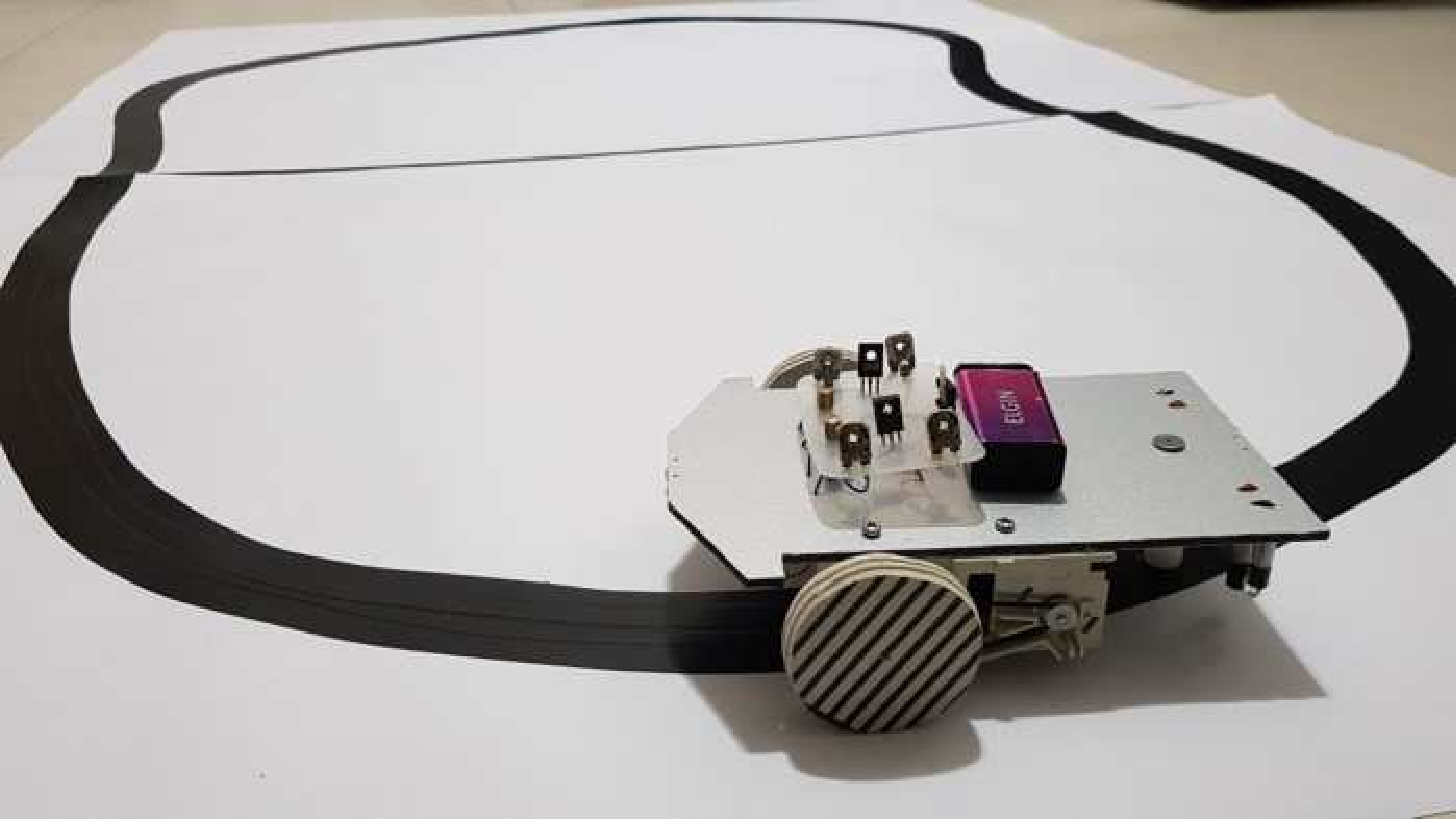
\includegraphics[width=0.5\textwidth]{figure-28.pdf}
\caption{Pista com fita dupla de 3.21m.}
\label{fig18}
\source{Acervo dos autores.}
\end{figure}

\item Solicite que determinem, empiricamente, o comprimento da trajetória em metros e centímetros (3,21m ou 321cm).
\item Requisite que cada estudante/grupo teste seu robô e determine o tempo gasto para percorrer o trajeto (6,42s).
\item Fale sobre velocidade média e induza-os a concluir qual é a velocidade média do AGV em cm/ms, m/s e cm/min (0,0005m/ms, 0,5m/s, 3000cm/min).
\item Relembre qual o comprimento da circunferência da roda (15,7cm) e solicite
que calculem quantos giros da roda serão necessários para percorrer o trajeto
(321cm e 20,44 giros).
\item\label{itm6} Relembre a velocidade média do robô em cm/min e faça-os calcular quantas
RPM a roda fará 
$$ 
\frac{3000}{15,7} \approx 191 \textmd{RPM}.
$$
Enfatize que esse foi o número de RPM da roda no teste.
\item Retome o item 3) da \Cref{sec-terceira} (245 RPM da roda). Ressalte a grande
perda de giro e levante as possíveis causas relatadas na mesma seção.
\item Faça uma abordagem sobre função inversa e coloque como desafio que os
estudantes calculem o número médio de RPM do motor a partir da distância
percorrida pelo AGV e do número de rotações da roda (191 RPM). Para resolver o
desafio deverão utilizar a função inversa de $f_2 \circ f_1$ (aplicada a 191
RPM, obtendo 2744 RPM).
\end{enumerate}


\subsection{Quinta atividade}\label{sec-quinta}
Nessa atividade é possível trabalhar torque, potência, proporcionalidade,
interpretação de dados e operações básicas. O objetivo é calcular o ganho de
torque na roda ($E_1$) com respeito à  $P_1$ e da $P_2$ com respeito ao motor
($P_1$).

\begin{enumerate}
\item Instigue os alunos sobre porque utilizar engrenagens/polias,
\Cref{fig17d}, ao invés de ligar as rodas diretamente aos motores. A mediação
da discussão deve ser feita de forma a concluir que, com o uso de
engrenagens/polias, ganha-se potência/força para movimentar o AGV.

\item Relembre que para $E_1$ dar um giro completo a $P_2$ precisa girar 4,285 voltas e conclua que
\begin{equation*}
2\pi R_{E1} = 4,285 (2\pi R_{P2}) \Rightarrow R_{E1} = 4,285 R_{P2}
\end{equation*}

\item Fale sobre velocidade angular ($\omega$ - grandeza que mede a rapidez com que é feito um percurso em sentido circular), velocidade tangencial ($V=R\omega$, onde $R$ é o raio da polia) e que em polias/engrenagens acopladas por correia as velocidades tangenciais são iguais.
\begin{equation*}
V_{P2} = V_{E1} \Leftrightarrow R_{P2} \omega_{P2} = R_{E1} \omega_{E1} \Leftrightarrow R_{P2} \omega_{P2} = 4,285 R_{P2} \omega_{E1} \Leftrightarrow \frac{\omega_{P2}}{\omega_{E_1}} = 4,285
\end{equation*}

\item Fale sobre torque, introduzindo a equação $P= T \omega$  ($P$ -- potência, $T$ -- torque e $\omega$ -- velocidade angular).

\item Explique que na transmissão da potência entre engrenagens há uma perda no deslizamento entre os dentes, que pode ser desconsiderada.

\item Assumindo a potência igual para $P_2$ e $E_1$, conclua que houve um ganho de $4,285$ de torque na $E_1$ com respeito ao torque da $P_2$.
\begin{equation*}
P_{E_1} = P_{P_2} \Leftrightarrow T_{E_1} = \frac{\omega_{P_2}}{\omega_{E_1}} T_{P_2} \Leftrightarrow T_{E_1} = 4,285 T_{P_2}
\end{equation*}

\item Realizando o mesmo estudo para $P_1$ e $P_2$, onde cada volta da $P_2$ corresponde a $3,343$ voltas da $P_1$, conclua que houve um ganho de $14,32$ de torque na roda ($E_1$) em relação ao torque do motor ($P_1$), conseguindo gerar força para deslocar o AGV no percurso.
\begin{equation*}
T_{P_2} = \frac{\omega_{P_1}}{\omega_{P_2}} T_{P_1} \Rightarrow T_{P_2} = 3,343 T_{P_1} \Rightarrow T_{P_1} \Rightarrow T_{E_1} = 4,285 T_{P_2} = 14,32 T_{P_1}
\end{equation*}

\end{enumerate}


Observação: Pode ser uma boa estratégia solicitar que sejam construídos robôs
com rodas de tamanhos diferentes para que possam investigar qual é a melhor
opção, para mais detalhes veja a \Cref{sec-experiencia}.



\section{Abordagens matemáticas possíveis a partir do estudo da parte eletrônica do AGV}\label{sec-abordagens}
Se for objetivo do professor aprofundar no estudo sobre o funcionamento do AGV,
seguem algumas atividades básicas. Estas atividades pressupõem o conhecimento
de alguns conceitos básicos de circuitos eletrônicos que não serão tratados
neste trabalho. Por exemplo, circuito eletrônico de corrente contínua, corrente
elétrica (unidade de medida Amperes (A) e é representada por $I$), fonte de
alimentação, potência (unidade de medida Watt (W) e é representada por $P$),
resistência elétrica (unidade de medida $\Omega$ (Ohm) e é representada por $R$), tensão
elétrica (unidade de medida Volt (V) e é representada por $V$) e lei de Ohm ($V = IR$). 
A seguir serão abordados alguns conceitos e resultados sobre circuitos
associados em série e em paralelo.


\subsection{Circuitos associados em série}\label{sec-circuitos}
Nessa atividade é possível trabalhar coleta de dados em esquemas, equações,
operações básicas, notação e significado de somatório. O objetivo é introduzir
algumas noções básicas sobre circuitos associados em série.

\begin{enumerate}
\item Introduza os circuitos associados em série, iniciando a representação por
meio de esquemas. Na \Cref{fig19} é possível visualizar um esquema de um
circuito com 4 resistores em série. Ressalte que podem ser colocados quaisquer
componentes eletrônicos no circuito.

\begin{figure}[H]
\centering
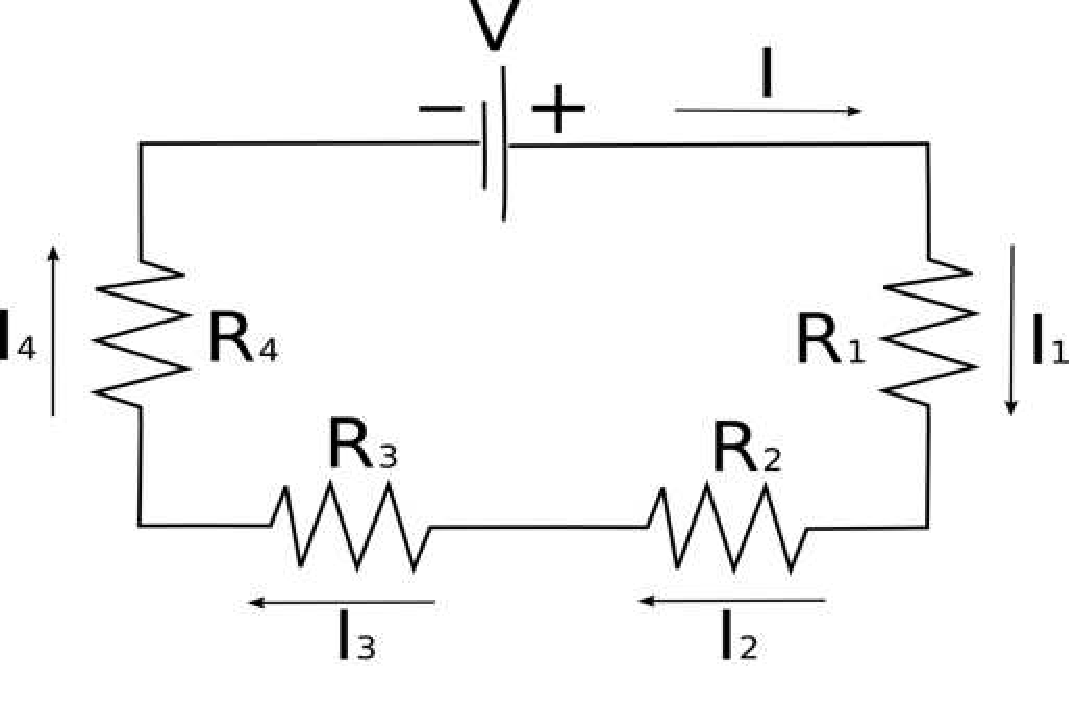
\includegraphics[width=0.5\textwidth]{figure-29.pdf}
\caption{Circuito associado em série.}
\label{fig19}
\source{Acervo dos autores.}
\end{figure}

\item Discuta a $2^a$ Lei de Kirchhoff (Lei das Malhas e suas consequências),
segundo a qual a soma algébrica das diferenças de potencial (ou tensão) de uma
malha é igual a zero e a corrente é igualmente distribuída em todos os
componentes no circuito.

\item Ilustre a referida lei a partir da \Cref{fig19}, concluindo que $V=V_1 +
V_2 + V_3 + V_4$, onde $V_i$ é a tensão no resistor $R_i$, para $i=1,2,3,4$.

\item Deduza que $I = I_1 = I_2 = I_3 = I_4$, com $I_i$ a corrente elétrica no
resistor $R_i$ , para $i=1,2,3,4$.

\item Argumente que, pela Lei de Ohm,
\begin{equation*}
RI = V = \sum_{i=1}^{4} V_i = \sum_{i=1}^{4} R_i I_i = \sum_{i=1}^{4} R_i I = I \sum_{i=1}^{4} R_i \Rightarrow R = \sum_{i=1}^{4} R_i
\end{equation*}

\item Generalize a fórmula para o caso n.

\end{enumerate}



\subsection{Circuitos associados em paralelo}\label{sec-circ-ass-p}

Nessa atividade é possível trabalhar coleta de dados em esquemas, equações,
operações básicas, notação e significado de somatório. O objetivo é introduzir
algumas noções básicas sobre circuitos associados em paralelo.


\begin{enumerate}
\item Introduza os circuitos associados em paralelo. Utilize, como exemplo, o
esquema da \Cref{fig20} de um circuito de 4 resistores em paralelo. Ressalte que
podem ser colocados quaisquer componentes eletrônicos no circuito que
continuarão valendo as conclusões.

\begin{figure}[h!]
\centering
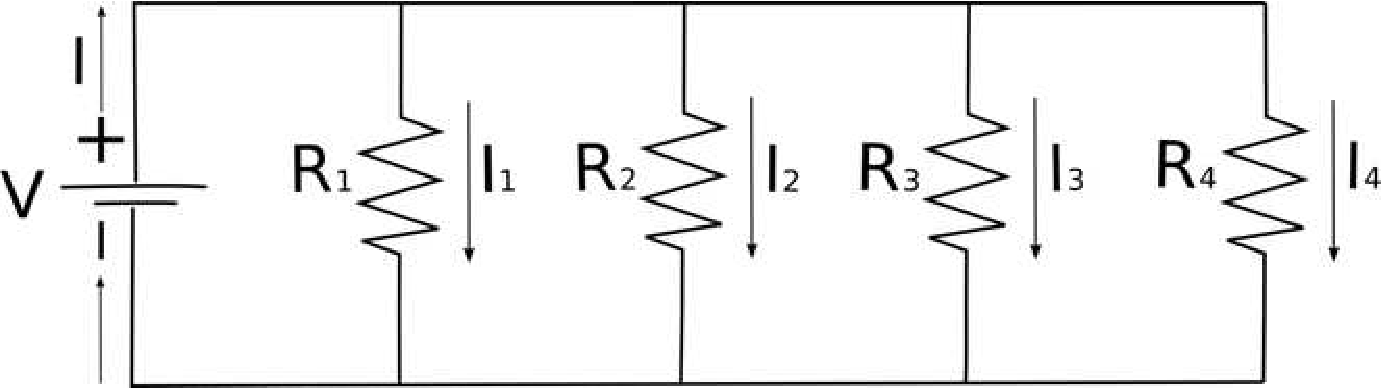
\includegraphics[width=0.6\textwidth]{figure-30.pdf}
\caption{Circuito associado em paralelo.}
\label{fig20}
\source{Acervo dos autores.}
\end{figure}

\item Discuta a $1^a$ Lei de Kirchhoff (Lei dos Nós), segundo a qual, em qualquer
nó, a soma das correntes que o deixam é igual à soma das correntes que chegam
até ele.

\item Ilustre a referida lei a partir da \Cref{fig20}, onde $I=I_1+I_2+I_3+I_4$.
\item Conclua que, $V=V_1=V_2=V_3=V_4$, pois estão conectados aos mesmos pontos.
\item Deduza, pela Lei de Ohm, que
\begin{equation*}
\frac{V}{R} = I = \sum_{i=1}^{4} I_i = \sum_{i=1}^{4} \frac{V_i}{R_i} = \sum_{i=1}^{4} \frac{V}{R_i} = V \sum_{i=1}^{4} \frac{1}{R_i} \Rightarrow \frac{1}{R} = \sum_{i=1}^{4} \frac{1}{R_i} .
\end{equation*}
\item Generalize a fórmula para o caso $n$.
\end{enumerate}


\subsection{Escolha do resistor}\label{sec-escolha-R}
Nessa atividade é possível trabalhar coleta de dados em esquemas, equações,
função linear, função exponencial e operações básicas. O objetivo nessa seção é
calcular a resistência máxima do resistor para não queimar o LED.

\begin{enumerate}
\item Esquematize o primeiro circuito, LED-resistor, conforme \Cref{fig21}, ressaltando a simbologia utilizada
\begin{figure}[h!]
\centering
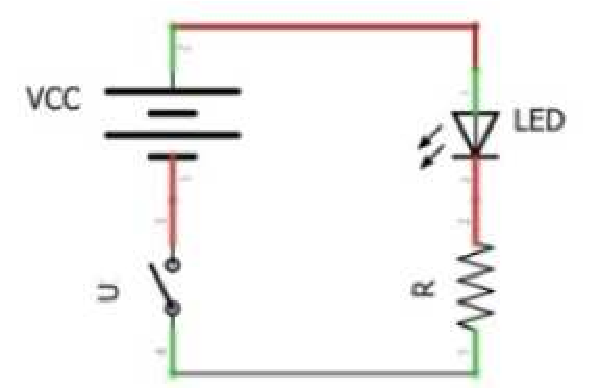
\includegraphics[width=0.3\textwidth]{figure-31.pdf}
\caption{Esquema do primeiro circuito.}
\label{fig21}
\source{Acervo dos autores.}
\end{figure}

\item Instigue os estudantes com a pergunta: sabendo a tensão na fonte (9V) e a
tensão do LED (3V), como escolher qual resistor utilizar de forma a evitar a
queima do LED?  Relembre que a corrente no LED é de $0,02$A.

\item Argumente que, por ser um circuito associado em série
\begin{equation*}
V_{FA} = V_{LED} + V_R \quad \textmd{e} \quad I = I_{LED} = I_R
\end{equation*}
em que, $V_{FA}$ -- tensão na fonte, $V_{LED}$ e $I_{LED}$ -- tensão e corrente no LED e $V_R$ e $I_R$ -- tensão e corrente no resistor.

\item Conclua, pela Lei de Ohm, que a resistência no resistor será
\begin{equation*}
R_R = \frac{V_R}{I_R} = \frac{V_{FA}-V_{LED}}{I_{LED}} = \frac{9-3}{0,02} = 300
\end{equation*}

\item Esclareça que resistores de $300\Omega$ não são comuns e que, neste caso,
será utilizado um resistor de $220\Omega$ e um de $100\Omega$ colocados em
série, os quais evitarão a queima do LED por ter uma resistência pouco maior do
que a calculada.

\item Explique que a resistência dos resistores é registrada por um código de
cores, conforme \Cref{fig22}, onde as primeiras três faixas indicam o valor
nominal e a última, a porcentagem que a resistência pode variar.

\begin{figure}[h!]
\centering
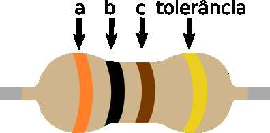
\includegraphics[width=0.2\textwidth]{figure-32.pdf}
\caption{Resistor de 4 cores.}
\label{fig22}
\source{Acervo dos autores.}
\end{figure}

\item Exponha que a função para encontrar o valor nominal do resistor de 4 cores é
\begin{equation*}
R(a,b,c) = (10a + b)10^c
\end{equation*}
E conclua quais cores devem ter as faixas, conforme \Cref{tab03} ($300\Omega =
R(3,0,1)= (10 \times 3+0)10^1$, ou seja, laranja, preto, marrom, o de
$220\Omega$ vermelho, vermelho, marrom e o de $100\Omega$ marrom, preto,
marrom). É uma oportunidade para abordar função exponencial.


\begin{table}[H]
\small
\caption{Tabela de cores: Valor nominal.}
\label{tab03}
\begin{tabularx}{\textwidth}{lllllllllll}
\toprule 
\multicolumn{11}{l}{Valor nominal} \\
\midrule
Cor & Preto & Marrom & Vermelho & Laranja & Amarelo & Verde & Azul & Violeta & Cinza & Branco \\
\midrule
Valor & 0 & 1 & 2 & 3 & 4 & 5 & 6 & 7 & 8 & 9 \\
\bottomrule
\end{tabularx}
\source{Acervo dos autores.}
\end{table}




\end{enumerate}




\subsection{Atividade final}\label{sec-atv-final}
Conhecendo o transistor, seu ganho beta (informado no datasheet), bem como o
motor e sua faixa de funcionamento (informado no datasheet), é possível
delimitar as resistências para o LDR e o potenciômetro que propiciam o
funcionamento dos motores. Além disso, medindo a resistência do LDR com um
multímetro, na pista proposta, pode-se delimitar faixas de resistência do
potenciômetro para o funcionamento dos motores. Nesta perspectiva, pode-se
confeccionar o circuito sem testes, bem como substituir os potenciômetros no
circuito LDR-potenciômetro por resistores. 

Como o objetivo deste artigo é propor atividades não muito complexas onde seja
possível evidenciar a Matemática subjacente, será proposta como atividade final
o cálculo da tensão no ponto de nó (teoria de divisão de tensão\footnote{Para
saber mais:
\url{https://pt.khanacademy.org/science/electrical-engineering/ee-circuit-analysis-topic/ee-resistor-circuits/a/ee-voltage-divider}.
Acesso em 02 de agosto de 2020.}), que no caso em tela é a tensão no
potenciômetro Vpot.

Nessa atividade é possível trabalhar coleta de dados em esquemas, equações,
sistema de equações lineares, funções e operações básicas. O objetivo é
calcular a tensão no ponto de nó LDR-potenciômetro-transistor, \Cref{fig23},
buscando determinar uma equação que relacione a tensão/corrente que vai para o
transistor com a tensão de entrada.

\begin{enumerate}
\item Esquematize o circuito, conforme \Cref{fig23}. Explique onde está o ponto
de nó e qual o objetivo.

\begin{figure}[h!]
\centering
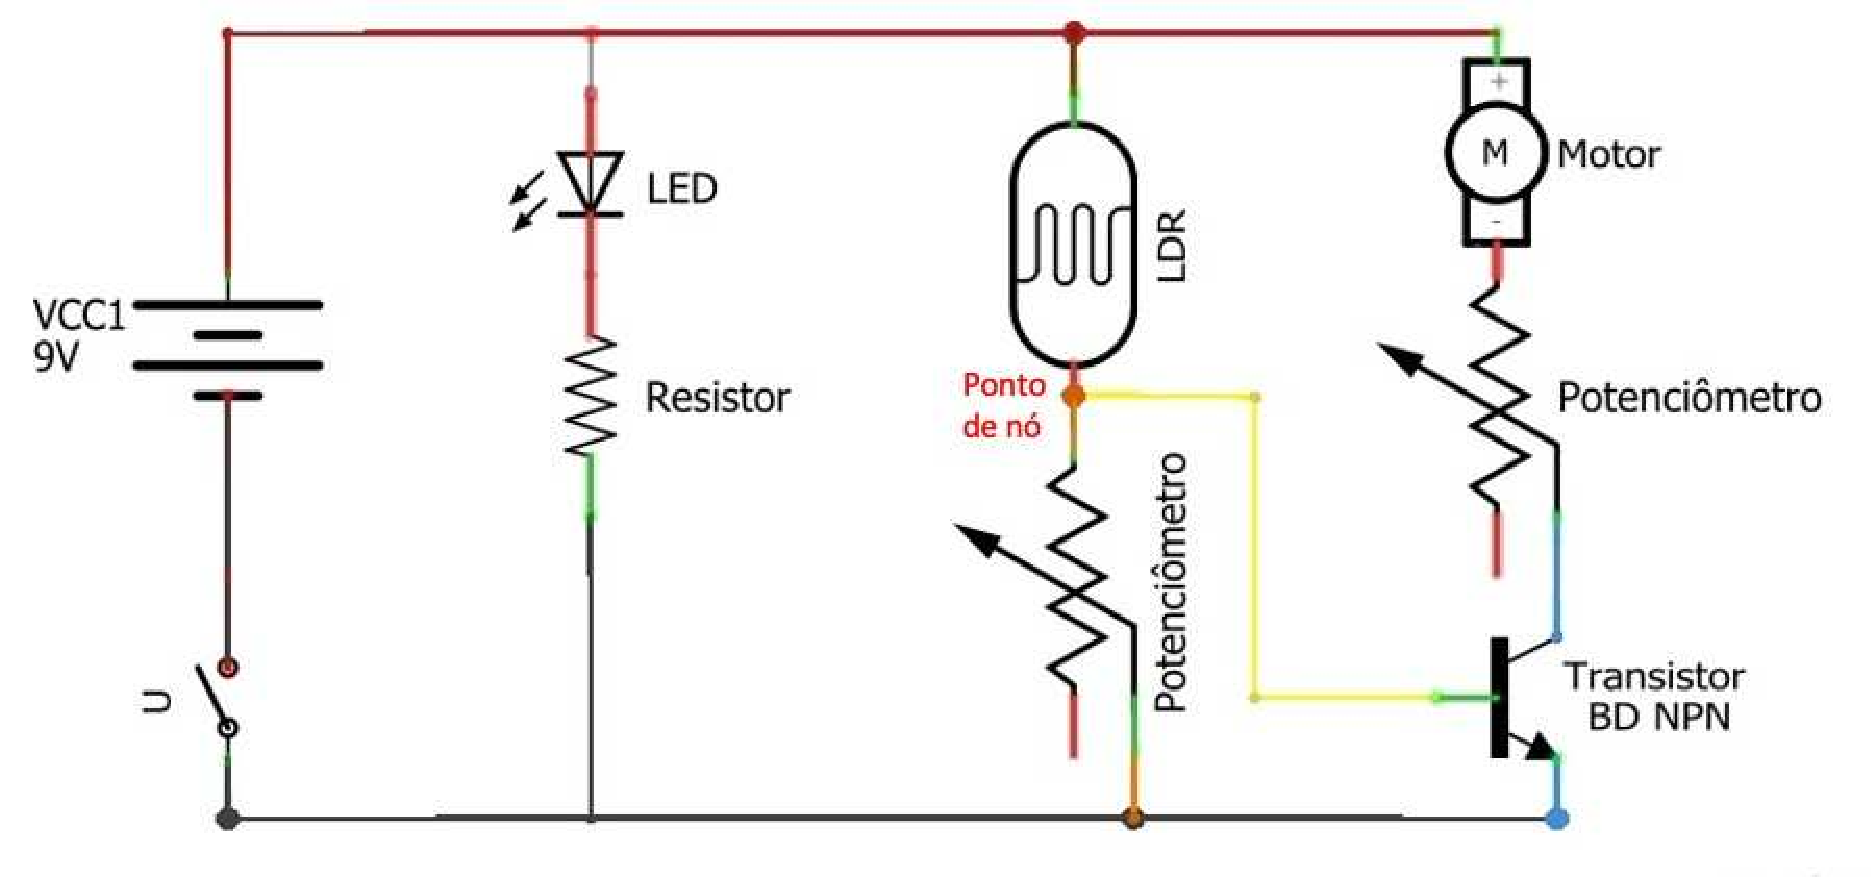
\includegraphics[width=0.6\textwidth]{figure-33.pdf}
\caption{Esquema do circuito do AGV.}
\label{fig23}
\source{Acervo dos autores.}
\end{figure}

\item Esquematize o segundo circuito, \Cref{fig24}. Ressalte que a tensão já
passou pela primeira resistência (LDR) e agora só depende da tensão que chega à
segunda (potenciômetro). A tensão no ponto de nó é igual à tensão do
potenciômetro.

\begin{figure}[h!]
\centering
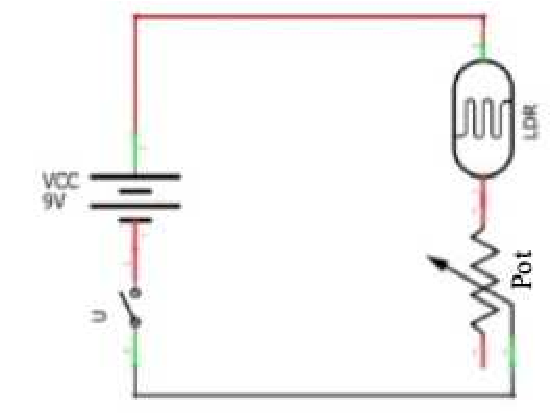
\includegraphics[width=0.3\textwidth]{figure-34.pdf}
\caption{Esquema do segundo circuito do AGV.}
\label{fig24}
\source{Acervo dos autores.}
\end{figure}

\item Comente que o circuito LDR-potenciômetro está em série, \Cref{fig24}, e por isso tem-se
\begin{equation*}
I_{LDR} = I_{pot}, \quad V = V_{LDR} + V_{pot} \quad \textmd{e} \quad R=R_{LDR} + R_{pot}
\end{equation*}

\item Utilize a lei de Ohm, para obter um sistema de equações lineares
\begin{equation*}
\begin{cases}
V_{FA} &= IR = I(R_{LDR}+R_{pot}) \\
V_{pot} &= I R_{pot}
\end{cases} 
\Rightarrow V_{pot} = \frac{R_{pot}}{R_{LDR} + R_{pot}} V_{FA}
\end{equation*}
Assim, é possível calcular a tensão no potenciômetro em função da tensão de
entrada e das resistências do potenciômetro e do LDR, sem conhecer a corrente
do potenciômetro. Para aplicar ao AGV construído, relembre que a fonte de
alimentação é de 9V e suponha que a resistência do potenciômetro deve ser
ajustada a $220\Omega$.

\item Substituindo os valores na fórmula, obtenha a tensão no potenciômetro em função da resistência do LDR 
$$ 
V_{pot} = \frac{220}{R_{LDR} + 220} 9 .
$$

\item Explique o resultado anterior abordando conceitos relativos a funções.

Agora é possível aplicar as relações obtidas nessa seção para a pista e AGV
construídos. É importante relembrar que a base da pista é clara e a trajetória
foi feita com uma fita isolante de cor preta (dupla) de $3,5$cm de largura.

\item Inicie a abordagem dividindo o estudo em três casos com respeito ao
posicionamento do LDR sobre a trajetória, conforme a \Cref{fig25}.

\begin{figure}[h!]
\centering
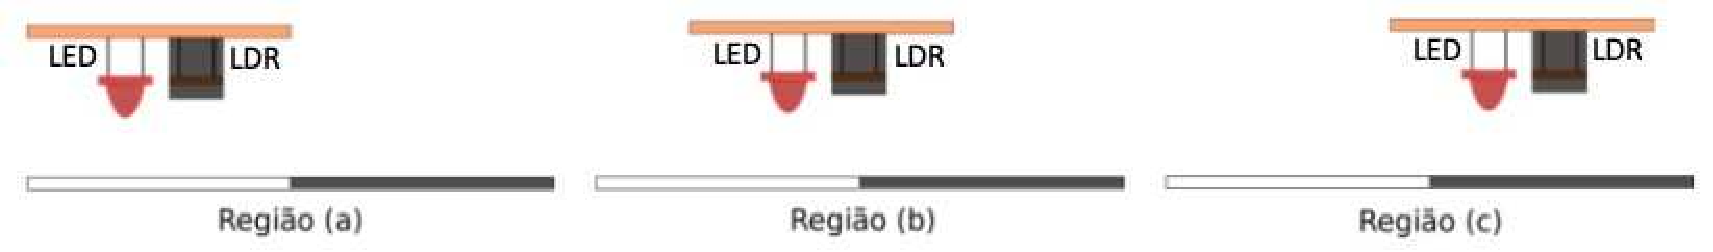
\includegraphics[width=0.8\textwidth]{figure-35.pdf}
\caption{Posicionamento do LDR sobre a trajetória.}
\label{fig25}
\source{Acervo dos autores.}
\end{figure}

\item Solicite que os estudantes façam a leitura das resistências dos LDR
conforme regiões definidas na \Cref{fig25} com um multímetro\footnote{Veja em:
\url{https://www.youtube.com/watch?v=XW2ZBwCD9dI}.}.

\item Faça com que os estudantes calculem o $V_{pot}$, para $R_{pot} = 220\Omega$ (faixa do transistor NPN
BD) e para $R_{pot} = 470 \Omega$ (faixa do transistor NPN TIP). Para direcionamento, considerando
altura do LDR do chão igual a 1cm, a iluminação com um LED de 3V a uma altura
de 1cm do chão e distante 1cm do LDR e $V_{FA}=9V$, serão obtidos os valores da \Cref{tab04}:

\end{enumerate}

\begin{sidewaystable}[ph]
\small
\centering
\vspace{-3cm}
\caption{Aplicação da Lei de Zipf nos documentos de Engenharia Elétrica e de Computadores.}
\label{tbl04}
\begin{tabular}{lp{0.3\textwidth}llllll}
\\
\toprule
\textbf{Forma} & \textbf{Características institucionais} & \textbf{Classificação} & \textbf{Forma associada} & \textbf{Classificação} & \textbf{Classe 1} & \textbf{Classe 2} & \textbf{Classe 5} \\
\midrule
\multirow{5}*{\textbf{Formação}} & 
    \multirow{5}{=}{\setlength\parskip{\baselineskip}%
    Atuam no 4º. estágio de decisão, o de implementação. A tendência é de um
    avanço de estágio, na direção da confirmação, o último estágio do processo
    de decisão da inovação, no sentido de consolidação como difusor da inovação
    no curso.}
& \multirow{5}*{\textit{Driver}} & & & -3,488 & \textbf{16,917} & 1,033 \\
 & & & \textbf{Conhecimento} & \textit{outcome} & -2,373 & \textbf{10,276} & -0,447 \\
 & & & \textbf{Científico} & \textit{outcome} & -3,488 & \textbf{11,783} & 0,091 \\
 & & & \textbf{Tecnológico} & \textit{outcome} & -0,771 & \textbf{3,339} & 0,348 \\
 & & & \textbf{Unidade curricular} & \textit{outcome} & 0,652 & \textbf{2,606} & -1,522 \\
 & & & & & & \\
 \midrule
\multirow{5}*{\textbf{Desenvolvimento}} & 
    \multirow{5}{=}{\setlength\parskip{\baselineskip}%
    Práticas institucionais isomórficas que posicionam o curso como semelhante
    à IES de referência no espaço europeu. Semelhante à perceção de  Formação e
    Competência}
 & \multirow{5}*{\textit{Driver}} & & & -0,678 & \textbf{26,88} & -2,581 \\
 & & & \textbf{Desempenho} & \textit{outcome} & -1,033 & \textbf{6,328} & -1,006 \\
 & & & \textbf{Investigação} & \textit{outcome} & -2,373 & \textbf{31,782} & -2,313 \\
 & & & & & & \\
\midrule
\multirow{5}*{\textbf{Competência}} & 
    \multirow{5}{=}{\setlength\parskip{\baselineskip}%
    É o resultado percebido pelo mercado de trabalho, no sentido de atender às
    necessidades profissionais esperadas do engenheiro Eletrotécnico e de
    computadores. Alocado no limítrofe entre o 4º. e o 5º. estágio de decisão
    de inovação.}
 & \multirow{5}*{\textit{Driver}} & & & -2,079 & \textbf{40,93} & -4,239 \\
 & & & \textbf{Ensino} & \textit{outcome} & -2,079 & \textbf{15,432} & 1,404 \\
 & & & \textbf{Aprendizagem} & \textit{outcome} & -0,678 & \textbf{19,483} & -0,635 \\
 & & & \textbf{Desenvolver} & \textit{outcome} & -0,771 & \textbf{10,328} & -0,752 \\
 & & & \textbf{Adquirir} & \textit{outcome} & -1,296 & \textbf{17,359} & -1,263 \\
 & & & & & & \\
\midrule
\multirow{2}*{\textbf{Ciclo de estudos}} &
    \multirow{2}{=}{\setlength\parskip{\baselineskip}%
    Adoção de práticas isomórficas de legitimação do curso perante a comunidade acadêmica, científica e pelos usuários}
 & \multirow{2}*{\textit{Driver}} & & & -4,853 & 1,073 & \textbf{38,01} \\
 & & & \textbf{Unidades curriculares} & \textit{outcome} & -0,049 & -1,81 & \textbf{8,486} \\
  & & & & & & \\
\midrule
\multirow{3}*{\textbf{Novo}} & 
    \multirow{3}{=}{\setlength\parskip{\baselineskip}%
    Driver da decisão de inovação no estágio intermediário entre a persuasão e a decisão de adoção pelo curso}
 & \multirow{3}*{\textit{Driver}} & & & -2,926 & -0,136 & \textbf{13,905} \\
 & & & \textbf{Querer} & \textit{outcome} & -1,296 & -0,022 & \textbf{11,623} \\
 & & & \textbf{Realizar} & \textit{outcome} & 3,389 & -0,718 & \textbf{3,56} \\
   & & & & & & \\
\midrule
\multirow{2}*{\textbf{Tecnologia}} & 
    \multirow{2}{=}{\setlength\parskip{\baselineskip}%
    Arranjo organizacional padronizado baseado em isomorfismo institucional}
 & \multirow{3}*{\textit{Driver}} & & & -0,771 & -0,893 & \textbf{12,277} \\
 & & & \textbf{Projecto educativo} & \textit{outcome} & -1,296 & -0,022 & \textbf{11,623} \\
   & & & & & & \\
\midrule
\multirow{3}*{\textbf{UC}} &
    \multirow{3}{=}{\setlength\parskip{\baselineskip}%
    Regras,normas e modelos isomórficos semelhantes ào de outros cursos}
 & \multirow{3}*{\textit{Driver}} & & & \textbf{4,484} & -7,101 & -7,738 \\
 & & & \textbf{FUC} & \textit{outcome} & \textbf{70,039} & -7,475 & -6,288 \\
 & & & \textbf{Ficha de Unidade Curricular} & \textit{outcome} & \textbf{16,02} & -1,196 & -1,006 \\

\bottomrule
\end{tabular}
\source{dos autores}
\end{sidewaystable}



Assim, conclui-se a exposição de diversas atividades que evidenciam a
Matemática e a Física, as quais podem ser executadas durante a construção do
AGV. Espera-se que os leitores busquem outras abordagens e compartilhem suas
experiências.



\section{Uma Experiência com diferentes AGV}\label{sec-experiencia}

Este trabalho foi elaborado tendo como base o AGV retratado nas
\Cref{fig14,fig16}. Um exemplar, \Cref{fig26}, foi construído, anteriormente,
com alguns componentes diferentes.

\begin{figure}[h!]
\begin{minipage}{0.47\textwidth}
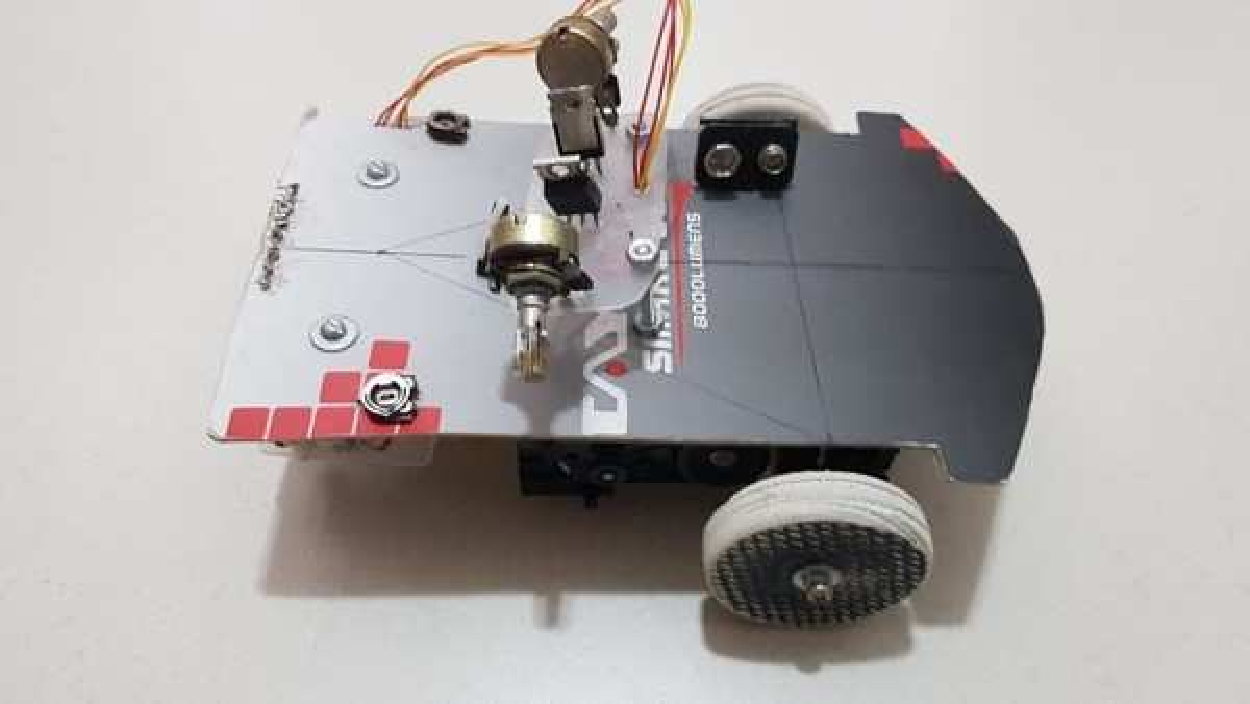
\includegraphics[width=\linewidth]{figure-36.pdf}
\subcaption{}
\end{minipage}
\hfill
\begin{minipage}{0.47\textwidth}
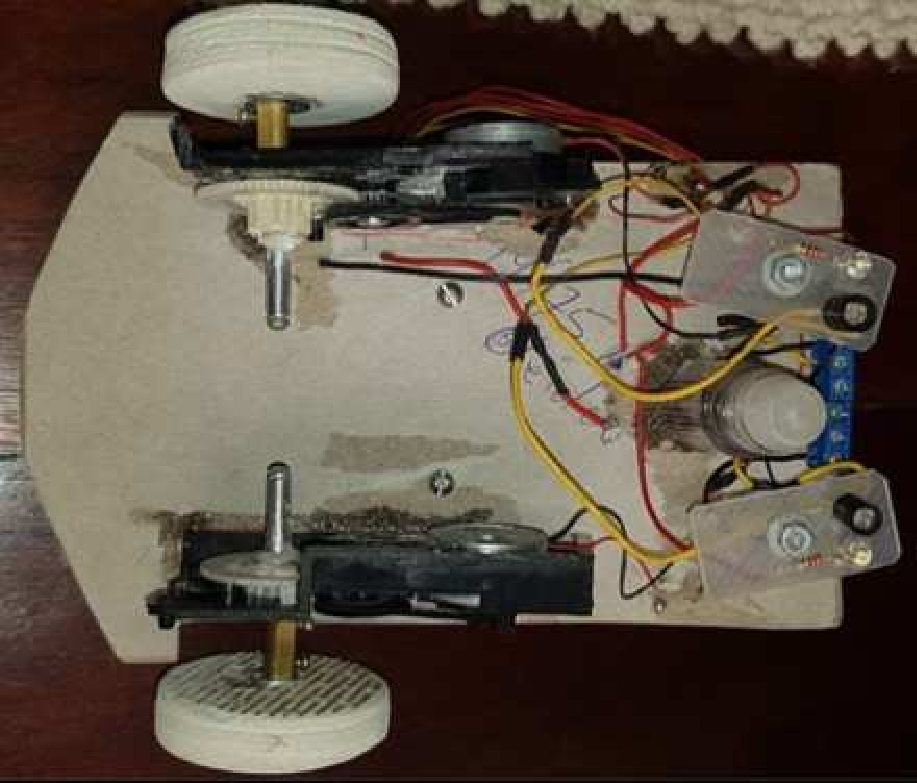
\includegraphics[width=\linewidth]{figure-37.pdf}
\subcaption{}
\end{minipage}
\caption{Primeiro exemplar (AGV).}
\label{fig26}
\source{Acervo dos autores.}
\end{figure}

Com o objetivo de estimular diferentes experiências, nessa seção são relatadas
as diferenças na construção dos exemplares e qual foi o impacto na velocidade e
precisão deles.

\begin{table}[htpb]
\caption{Componentes do primeiro e segundo exemplares do AGV.}
\label{tab05}
\begin{tabular}{@{}
   >{\raggedright\arraybackslash}p{0.45\textwidth}
   >{\raggedright\arraybackslash}p{0.45\textwidth}
@{}}
\toprule 
AGV segundo Exemplar & AGV primeiro Exemplar \\
\midrule
\multicolumn{2}{c}{Roda dianteira de roll-on labial} \\
\multicolumn{2}{c}{Roda traseira de chinelo} \\
\multicolumn{2}{c}{Placa para fixar componentes de pasta de plástico} \\
\multicolumn{2}{c}{1 resistor de $220\Omega$ e 1 resistor de $100\Omega$ (em série)} \\
\multicolumn{2}{c}{LED de alto brilho de luminária de Emergência de 3V} \\
\multicolumn{2}{c}{LDR 5mm} \\
\multicolumn{2}{c}{Chave (liga/desliga)} \\
\multicolumn{2}{c}{Clip conector de bateria 9v} \\
\midrule
Chassi de ACM & Chassi de capa rígida de caderno \\
Transistor NPN BD135 & Transistor PNP TIP 105 \\
Motores de leitora de DVD de computador, de 3520RPM, com engrenagens (60 e 14 dentes) e polias & Motores de aparelho de DVD, de 3520RPM,com engrenagens (64 e 14 dentes) e polias \\
2 Potenciômetros trimpot $500\Omega$ para regular as velocidades dos motores & 2 Potenciômetro trimpot $2K\Omega$ para regular as velocidades dos motores \\
2 Potenciômetros trimpot $5K\Omega$ ($120\Omega$ à $330\Omega$)para regular as correntes para as bases dos transistores & 2 Potenciômetros $10K\Omega$ ($200\Omega$ à $600\Omega$) para regular as correntes para as bases dos transistores \\
\bottomrule
\end{tabular}
\source{Acervo dos autores.}
\end{table}




A mesma análise em relação ao número de RPM da roda versus o número de RPM do
motor pode ser realizada para o primeiro AGV. Como a única alteração
determinante ocorreu na engrenagem $E1$ (64 dentes e 60 dentes), a função
definida no \Cref{itm1sec423} da \Cref{sec-terceira} para o primeiro AGV é 
\begin{align*}
h: \mathbb{R}^{+} &\rightarrow \mathbb{R}^{+} \\
  x &\rightarrow 0,0654 x \nonumber
\end{align*}

Como o número de rotações do motor é o mesmo para ambos os robôs, 3520 RPM,
tem-se 230 RPM para as rodas do primeiro AGV. Nos testes realizados no
percurso, o primeiro AGV percorreu a pista de 3,21m em 6,73s, ou seja, com
velocidade média de 0,476m/s ou 2.861cm/min. Na prática, como a roda do
primeiro AGV possui 2,37cm e seu comprimento de arco é 14,9cm, considerando as
perdas ocorridas no percurso, obtém-se, aproximadamente, 192RPM para a roda. A
\Cref{tab06} é um comparativo entre os dois AGV, cujos valores (exceto raio e peso)
foram obtidos pela média feita a partir de vários testes.

\input{table06.tex}

É importante salientar que a perda de RPM no percurso foi maior para o
transistor BD135 (de 245 para 191) em comparação com o transistor TIP 105 (230
para 192). Portanto, o TIP105 teve uma resposta melhor na correção do AGV. Além
disso, o tamanho da roda influenciou na velocidade do robô, pois mesmo com um
número menor de rotações da roda (191RPM), o segundo AGV obteve velocidade
maior que o primeiro (192RPM para roda).

Portanto, as escolhas dos componentes e circuitos podem induzir a construção de
um AGV mais rápido ou mais lento, mais preciso ou não. Assim, a proposta de uma
competição pode ser interessante, dependendo do contexto em que estiver sendo
feita esta abordagem. Porém, ressalta-se a importância da valorização não
somente do robô mais preciso e veloz nessa competição, mas de todos os
participantes que discutirem e apresentarem propostas, enfatizando o
aprendizado e conhecimento construídos. O mais importante é incentivar a
colaboração.


\section{Considerações finais}\label{sec-considera}
O desenvolvimento de um projeto com RE dessa magnitude é um caminhar ao
desconhecido, pois toda ação implica em uma nova descoberta, a qual proporciona
um aprendizado. Desta forma, a execução do projeto é similar a um processo de
resolução de problemas. E até mesmo após a finalização do projeto continuam
surgindo questões, pois há sempre o desejo de melhorar a criação. Nesta busca
pela perfeição, a Matemática torna-se aliada no processo de interpretação dos
resultados obtidos pelo robô, orientando desde o design até a escolha dos
objetos para construí-lo.

No contexto atual, de produção e consumo tecnológico, estamos produzindo muito
lixo eletrônico. Logo, o trabalho com robótica utilizando sucata constitui-se
uma oportunidade de aprendizagem interdisciplinar, abordando questões
ambientais. Reaproveitar eletrônicos para construção de robôs abre um leque de
possibilidades educativas, com o desenvolvimento de uma consciência quanto ao
consumo e ao meio ambiente, podendo ser construídas propostas envolvendo
diversos temas transversais no ensino.

Ensinar Matemática de forma que seja compreendida e não venha causar uma fobia
é um desafio no processo de educação Matemática. As tecnologias digitais
possibilitam um trabalho com conteúdos da disciplina que atrai os estudantes,
pois elas já fazem parte da cultura digital de crianças e jovens. Construir um
robô é um trabalho divertido e quando aliamos à Matemática estamos agregando
maior conhecimento e domínio sobre a tecnologia. O que buscamos é “que os
jovens de hoje, consumidores de tecnologias, possam ser mais: mais produtores,
mais críticos, mais criativos, mais preocupados com os problemas locais,
regionais e até globais” \cite[p. 286]{barbosa2016}.

Com RE usando de materiais livres fomenta-se uma robótica mais inclusiva e
acessível, tendo em vista que materiais comercializados para fins educacionais
têm um valor muito além das condições de muitas instituições de ensino
públicas. Isto posto, neste artigo aborda-se uma visão de estudos de
dispositivos mecânicos e eletrônicos, a partir de conceitos matemáticos,
evidenciando como ela auxilia no processo de construção de um robô, utilizando
sucata, e seu aperfeiçoamento. Propicia-se, assim, a elaboração de
conhecimentos matemáticos em um ambiente motivador e prazeroso. Mais que
ensinar Matemática, é fazer deste conhecimento fundamental e em evolução, um
instrumento de transformação e leitura do mundo em que vivemos.

Em trabalhos posteriores, pretende-se aprofundar no estudo de dispositivos
mecânicos e eletrônicos, a partir de conceitos matemáticos, com a finalidade de
ampliar a gama de opções de mecanismos que podem ser usados para construção de
robôs seguidores de linha. Além disso, objetiva-se iniciar o trabalho com
microcontroladores reprogramáveis para a inserção do controle remoto no robô e
introdução de programação para o público-alvo. Ademais, devem ser realizadas
experimentações das atividades propostas a fim de verificar suas contribuições
para a aprendizagem dos envolvidos.


\printbibliography\label{sec-bib}
% if the text is not in Portuguese, it might be necessary to use the code below instead to print the correct ABNT abbreviations [s.n.], [s.l.] 
%\begin{portuguese}
%\printbibliography[title={Bibliography}]
%\end{portuguese}


\end{document}
